\section{Durable model}\label{sec:DurableModel}

The second example is a consumption-savings model with durable and nondurable goods. It is a simplified version of the model in \cite{Monninger2025-cz} which uses endogeneous search as a numerical tool to solve the model. This section focuses on the solution method and compares the usage of taste shocks, endogeneous search, and stochastic durable prices.

\subsection{Model setup}\label{sec:ModelBasic}
The model consists of ex-ante identical agents who face uninsurable income risk and can consume non-durable goods, receive flow utility from a durable good, and can save in one single risk-free liquit asset.

\begin{figure}[h!]
	\centering
	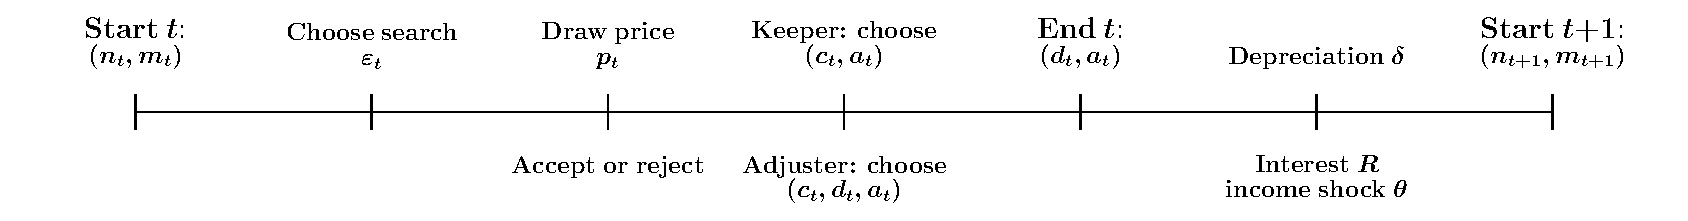
\includegraphics[width=\textwidth]{timeline_DurableModel.pdf}
	\caption{Timeline of the durable model}
	\label{fig:timeline_DurableModel}
\end{figure}

The agent starts each period with beginning-of-period durable stock ($n_t$) and market resources ($m_t$). The agent solves the adjuster and keeper problems separately and chooses optimal levels of nondurable consumption $c_t$, durable stock $d_t$, and assets $a_t$. The discrete keep-versus-adjust decision is then resolved by a hard maximum over the two conditional value functions. At the end of the period, the agent holds a durable stock $d_t$ and liquid assets $a_t$. Between period $t$ and $t+1$, the transitory income shock materializes, interest is received, and the durable stock depreciates.

Each household is characterized by two state variables: beginning-of-period market resources $m_t$ and the stock of durables $n_t$. Preferences exhibit constant relative risk aversion and combine nondurable consumption $c_t$ and the service flow of durables $d_t$ using a Cobb-Douglas aggregator\footnote{Using this form is standard (eg see \cite{Berger2015-kp, McKay2021-ib}) which is in line with micro-evidence \cite{Berger2018-yb}. An alternative approach is to use a CES aggregator as in \cite{Mankiw1983-za}}:
\begin{align}
	u(c_t, d_t) &= \frac{\big(c_t^\alpha d_t^{1-\alpha}\big)^{1-\rho}}{1-\rho}, \qquad \alpha \in (0,1), \ \rho > 0.
\end{align}

At the start of the period, the household observes $(m_t, n_t)$ and decides whether to keep the durable stock unchanged or to adjust. If no adjustment occurs, the household sets $d_t = n_t$ and allocates $m_t$ between nondurable consumption and savings. If the household adjusts, it sells the entire beginning-of-period stock at no price risk but incurs a proportional adjustment cost $\tau \in (0,1)$. The resulting liquidity is
\begin{align}
	\ell_t = m_t + (1-\tau)n_t,
\end{align}
which can then be allocated across nondurable consumption, a new durable stock $d_t$, and savings $a_t$.

The household's problem is the hard discrete choice between keeping and adjusting:
\begin{align}
	v_t(m_t,n_t) = \max\Big\{ v_t^{\text{keep}}(m_t,n_t),\; v_t^{\text{adj}}(\ell_t)\Big\},
\end{align}
where $v_t^{\text{keep}}$ and $v_t^{\text{adj}}$ are the value functions conditional on keeping or adjusting.

Labor income is idiosyncratic and purely transitory. Normalized income is
\begin{align}
	y_t = \theta_t,
\end{align}
where $\theta_t$ is i.i.d.\ log-normally distributed with $\mathbb{E}[\theta_t] = 1$ and a strictly positive standard deviation. There is no unemployment risk.

Assets earn a single interest rate $r$, so the gross interest factor is $\mathcal{R} = 1+r$. The durable stock depreciates at rate $\delta \in (0,1)$. There are no maintenance costs and no operation costs. Therefore, next-period states evolve according to
\begin{align}
	m_{t+1} &= \mathcal{R} a_t + \theta_{t+1},\\
	n_{t+1} &= (1-\delta)\, d_t.
\end{align}

Borrowing is prohibited: the loan-to-value ratio is zero and the lower bound on assets is $\underline{a}=0$, so end-of-period assets must satisfy $a_t \ge 0$.

Hence, the Bellman equations conditional on keep and adjust are:
\begin{align}
	v_t^{\text{keep}}(m_t,n_t) &= \max_{c_t} \ u(c_t ,d_t) + \beta \mathbb{E}_t \big[ v_{t+1}(m_{t+1},n_{t+1}) \big],\\
	& \text{s.t. } a_t = m_t - c_t \geq 0,\\
	& \qquad d_t = n_t,\\
	& \qquad m_{t+1} = \mathcal{R} a_t + \theta_{t+1},\\
	& \qquad n_{t+1} = (1-\delta)\, d_t.\\[1em]
	v_t^{\text{adj}}(\ell_t) &= \max_{c_t,d_t} \ u(c_t,d_t) + \beta \mathbb{E}_t \big[ v_{t+1}(m_{t+1},n_{t+1}) \big],\\
	& \text{s.t. } a_t = \ell_t - c_t - d_t \geq 0,\\
	& \qquad m_{t+1} = \mathcal{R} a_t + \theta_{t+1},\\
	& \qquad n_{t+1} = (1-\delta)\, d_t.
\end{align}

With the following first-order conditions with respect to nondurable consumption and durable stock:
\begin{align}
	\frac{\partial v_t^{adj}}{\partial c_t} &= u_c(c_t, d_t) \geq \beta \mathcal{R}\, \mathbb{E}_t \big[v_{t+1}^m\big], \label{eq:FOC_c_basic} \\
	\frac{\partial v_t^{adj}}{\partial d_t} &= u_d(c_t, d_t) \geq \beta \mathcal{R}\, \mathbb{E}_t\big[v_{t+1}^m\big] - \beta (1 - \delta)\, \mathbb{E}_t\big[v_{t+1}^n\big], \label{eq:FOC_d_basic}
\end{align}

Equations~\ref{eq:FOC_c_basic} and~\ref{eq:FOC_d_basic} are stated as KKT conditions. Equality holds when the borrowing constraint does not bind, and the left-hand side strictly exceeds the right-hand side when it does. Equation~\ref{eq:FOC_c_basic} equates the marginal utility of nondurable consumption with the discounted shadow value of savings. Equation~\ref{eq:FOC_d_basic} shows that the marginal utility of durables equals the net user cost: the first term on the right is the discounted opportunity cost $\mathcal{R}$ of diverting a unit of resources into durables rather than liquid assets, and the second term is the discounted benefit of carrying the remaining durable stock $(1-\delta)d_t$ into the next period.

\subsection{Algorithm}\label{subsec:AlgorithmBasic}
This section outlines the algorithm for one recursive period of the baseline model: no Extreme Value Type~I taste shocks, no directed search, and no durable-price dispersion. The discrete keep-versus-adjust choice is resolved by a hard maximum. The terminal period is closed form---the keeper sets $c_T=m_T$ and $d_T=n_T$, the adjuster sets $c_T=\alpha\ell_T$ and $d_T=(1-\alpha)\ell_T$, and the two branches are combined by a hard max---so Algorithm~\ref{alg:durable_baseline} starts from a given next-period solution $(v_{t+1},\,v_{t+1}^{m},\,v_{t+1}^{n})$.

Define the end-of-period (gothic) objects on $(d_t,a_t)$ by
\begin{align}
	\mathfrak{v}_c'(d_t,a_t) &= \beta\,\mathcal{R}\,\mathbb{E}_t\big[v_{t+1}^{m}(n_{t+1},m_{t+1})\big],\\
	\mathfrak{v}_d'(d_t,a_t) &= \beta\,(1-\delta)\,\mathbb{E}_t\big[v_{t+1}^{n}(n_{t+1},m_{t+1})\big],\\
	\mathfrak{v}(d_t,a_t) &= \beta\,\mathbb{E}_t\big[v_{t+1}(n_{t+1},m_{t+1})\big],
\end{align}
with $m_{t+1}=\mathcal{R}a_t+\theta_{t+1}$ and $n_{t+1}=(1-\delta)d_t$. The expectation over $\theta_{t+1}$ may be evaluated by quadrature (as written below) or by the transition-matrix integration described in Appendix~\ref{sec:appdx_model_basic}. Because adjustment costs make the first-order conditions only necessary, the keeper step applies a DC-EGM upper envelope \citep{Iskhakov2017-jb} and the adjuster step applies FUES \citep{Dobrescu2022-ii}.

\begin{algorithm}[htbp]
\caption{EGM step for the baseline durable model (hard max)}
\label{alg:durable_baseline}
\DontPrintSemicolon
Let $\vec{\theta}=\{\theta_1,\dots,\theta_J\}$ be quadrature points for the transitory income shock with weights $\vec{\omega}=\{\omega_1,\dots,\omega_J\}$.\;
Form ascending grids $\vec{a}_t=\{a^1,\dots,a^I\}$, $\vec{d}_t=\{d^1,\dots,d^L\}$, a fine durable grid $\vec{d}_t^{\mathrm{adj}}$ for the adjuster FOC scan, and beginning-of-period grids $\vec{n}_t$, $\vec{m}_t$.\;
\BlankLine
\tcc{End-of-period (gothic) functions}
\For{$i = 1,\dots,I$}{
	\For{$q = 1,\dots,L$}{
		\For{$j = 1,\dots,J$}{
			Compute $m_{t+1}^{j}(a^i)=\mathcal{R}a^i+\theta_j$ and $n_{t+1}(d^q)=(1-\delta)d^q$\;
			Interpolate $v_{t+1}$, $v_{t+1}^{m}$, and $v_{t+1}^{n}$ at $(n_{t+1}(d^q),\,m_{t+1}^{j}(a^i))$\;
		}
		Compute $\mathfrak{v}_c'(d^q,a^i)=\beta\mathcal{R}\sum_{j=1}^{J}\omega_j\,v_{t+1}^{m}(n_{t+1}(d^q),m_{t+1}^{j}(a^i))$\;
		Compute $\mathfrak{v}_d'(d^q,a^i)=\beta(1-\delta)\sum_{j=1}^{J}\omega_j\,v_{t+1}^{n}(n_{t+1}(d^q),m_{t+1}^{j}(a^i))$\;
		Compute $\mathfrak{v}(d^q,a^i)=\beta\sum_{j=1}^{J}\omega_j\,v_{t+1}(n_{t+1}(d^q),m_{t+1}^{j}(a^i))$\;
	}
}
\BlankLine
\tcc{Keeper: EGM with $d_t=n_t$, then DC-EGM upper envelope}
\For{each $n\in\vec{n}_t$}{
	\For{$i = 1,\dots,I$}{
		Compute $c_t^{\mathrm{keep}}(a^i;n)=u_c^{-1}\big(\mathfrak{v}_c'(n,a^i);\,n\big)$\;
		Compute endogenous resources $m_t^{\mathrm{EGM}}(a^i;n)=a^i+c_t^{\mathrm{keep}}(a^i;n)$\;
		Compute $v_t^{\mathrm{EGM}}(a^i;n)=u\big(c_t^{\mathrm{keep}}(a^i;n),n\big)+\mathfrak{v}(n,a^i)$\;
	}
	Apply a DC-EGM upper envelope to $\{(m_t^{\mathrm{EGM}},\,c_t^{\mathrm{keep}},\,v_t^{\mathrm{EGM}})\}$ and interpolate onto $\vec{m}_t$ to obtain $c_t^{\mathrm{keep}}(n,m)$, $a_t^{\mathrm{keep}}=\max\{m-c_t^{\mathrm{keep}},0\}$, and $d_t^{\mathrm{keep}}=n$\;
	Compute $v_t^{\mathrm{keep}}(n,m)=u(c_t^{\mathrm{keep}},n)+\mathfrak{v}(n,a_t^{\mathrm{keep}})$, $v_t^{m,\mathrm{keep}}=u_c(c_t^{\mathrm{keep}},n)$, and $v_t^{n,\mathrm{keep}}=u_d(c_t^{\mathrm{keep}},n)+\mathfrak{v}_d'(n,a_t^{\mathrm{keep}})$\;
}
\BlankLine
\tcc{Adjuster: FOC roots in $a$ on a fine $d$-grid, then FUES in liquidity}
Initialize empty candidate clouds for $(\ell_t,c_t,d_t,a_t,v_t)$\;
\For{each $d\in\vec{d}_t^{\mathrm{adj}}$}{
	Find all roots $a$ of $u_d(c,d)-\mathfrak{v}_c'(d,a)+\mathfrak{v}_d'(d,a)=0$ with $c=u_c^{-1}\big(\mathfrak{v}_c'(d,a);\,d\big)$\;
	\For{each root $a$}{
		Compute $\ell_t=a+c+d$ and $v_t^{\mathrm{adj}}=u(c,d)+\mathfrak{v}(d,a)$\;
		Append $(\ell_t,c,d,a,v_t^{\mathrm{adj}})$ to the candidate cloud\;
	}
}
Sort candidates by $\ell_t$ and apply FUES to obtain refined points $(\ell_t,c_t^{\mathrm{adj}},d_t^{\mathrm{adj}},a_t^{\mathrm{adj}},v_t^{\mathrm{adj}})$\;
Construct one-dimensional interpolants $c_t^{\mathrm{adj}}(\ell)$, $d_t^{\mathrm{adj}}(\ell)$, and $a_t^{\mathrm{adj}}(\ell)$\;
\For{each $(n,m)\in\vec{n}_t\times\vec{m}_t$}{
	Compute $\ell_t=m+(1-\tau)n$\;
	Evaluate $c_t^{\mathrm{adj}}(\ell_t)$, $d_t^{\mathrm{adj}}(\ell_t)$, and $a_t^{\mathrm{adj}}=\max\{\ell_t-c_t^{\mathrm{adj}}-d_t^{\mathrm{adj}},0\}$\;
	Compute $v_t^{\mathrm{adj}}(\ell_t)=u(c_t^{\mathrm{adj}},d_t^{\mathrm{adj}})+\mathfrak{v}(d_t^{\mathrm{adj}},a_t^{\mathrm{adj}})$, $v_t^{m,\mathrm{adj}}=u_c(c_t^{\mathrm{adj}},d_t^{\mathrm{adj}})$, and $v_t^{n,\mathrm{adj}}=(1-\tau)\,u_c(c_t^{\mathrm{adj}},d_t^{\mathrm{adj}})$\;
}
\BlankLine
\tcc{Hard-max discrete choice}
\For{each $(n,m)\in\vec{n}_t\times\vec{m}_t$}{
	Set $\mathcal{I}_t(n,m)=1$ if $v_t^{\mathrm{adj}}\big(m+(1-\tau)n\big)\ge v_t^{\mathrm{keep}}(n,m)$ and $0$ otherwise\;
	Set $(c_t,d_t,a_t,v_t,v_t^{m},v_t^{n})$ to the adjuster branch if $\mathcal{I}_t=1$ and to the keeper branch if $\mathcal{I}_t=0$\;
}
Collect the combined policies and (inverse) value functions on $(\vec{n}_t,\vec{m}_t)$ for use in period $t-1$.\;
\end{algorithm}

\subsection{Illustration of the numerical challenge}

Fig.~\ref{fig:baseline_T} illustrates the terminal solution. Taking the hard-max between the options of adjusting and keeping, the S,s structure emerges (fig.~\ref{fig:baseline_ss_T}) which leads to a sharp switch between fully adjusting or fully keeping. As a result, the optimal policy functions of the model conditional on adjusting and keeping experience discontinuities along the switchpoints as illustrated for the durable consumption function (fig.~\ref{fig:baseline_d_T}).

\begin{figure}[htbp]
	\centering
	\begin{subfigure}{0.48\textwidth}
		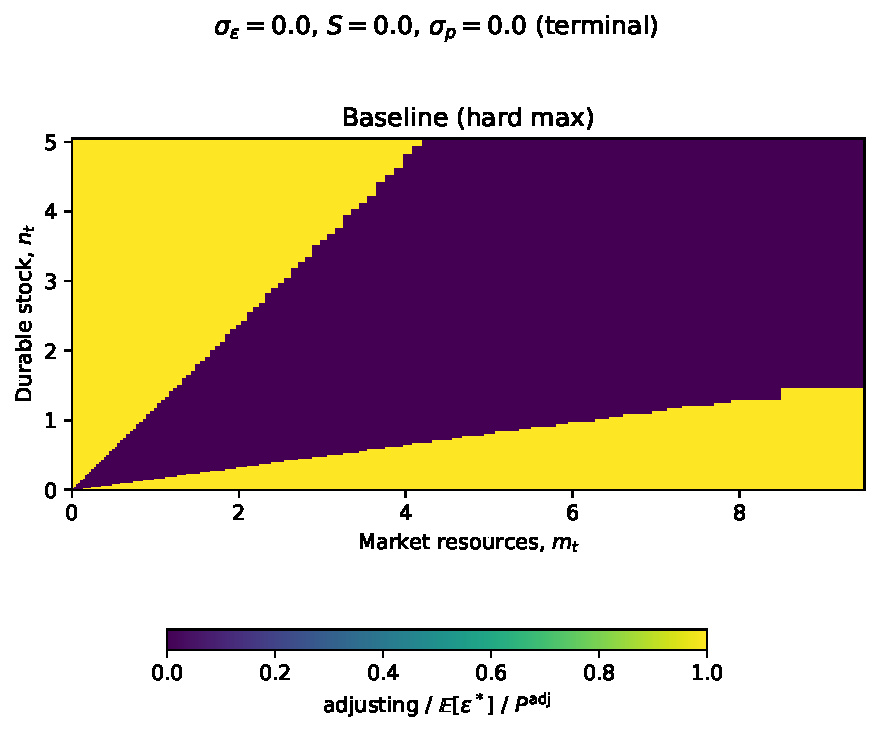
\includegraphics[width=\linewidth]{../Figures/DurableModel/Baseline_Ss_T.pdf}
		\caption{Adjustment region (S,s bands).}
		\label{fig:baseline_ss_T}
	\end{subfigure}
	\hfill
	\begin{subfigure}{0.48\textwidth}
		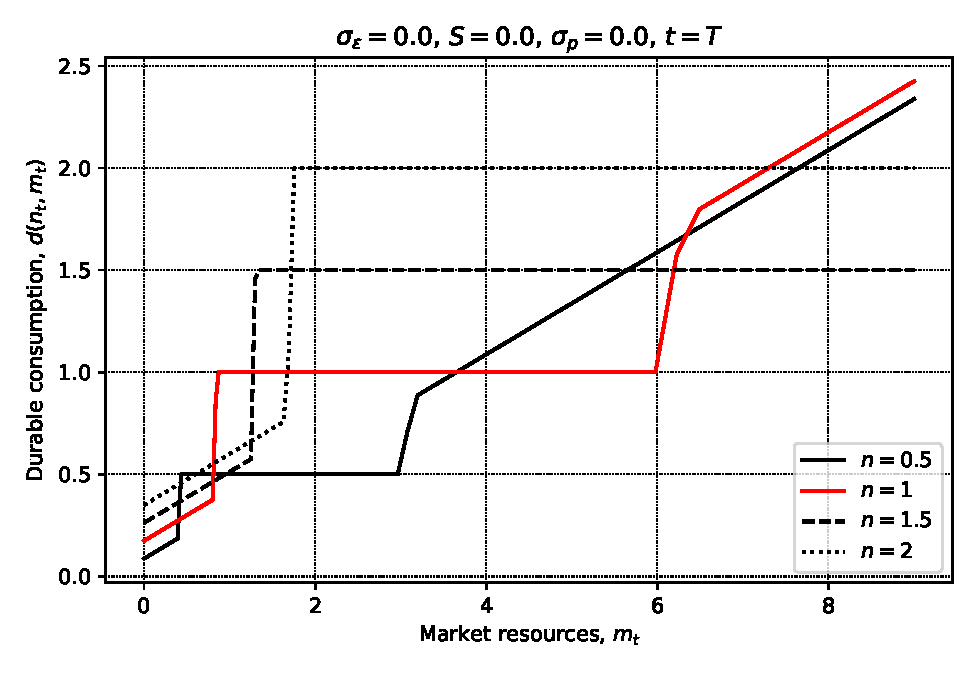
\includegraphics[width=\linewidth]{../Figures/DurableModel/Baseline_d_T.pdf}
		\caption{Durable policy $d_t(n_t,m_t)$.}
		\label{fig:baseline_d_T}
	\end{subfigure}
	\vspace{0.5em}
	\begin{subfigure}{0.48\textwidth}
		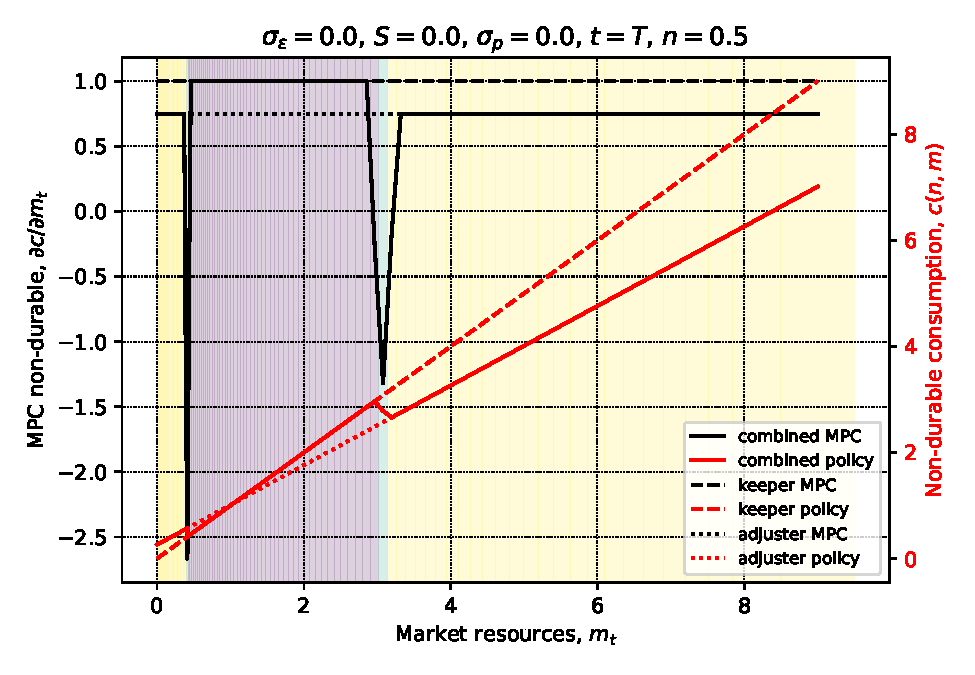
\includegraphics[width=\linewidth]{../Figures/DurableModel/Baseline_c_T_MPC_decomp.pdf}
		\caption{MPC decomposition of nondurable consumption $c_t(n_t,m_t)$.}
		\label{fig:baseline_c_T_MPC_decomp}
	\end{subfigure}
	\hfill
	\begin{subfigure}{0.48\textwidth}
		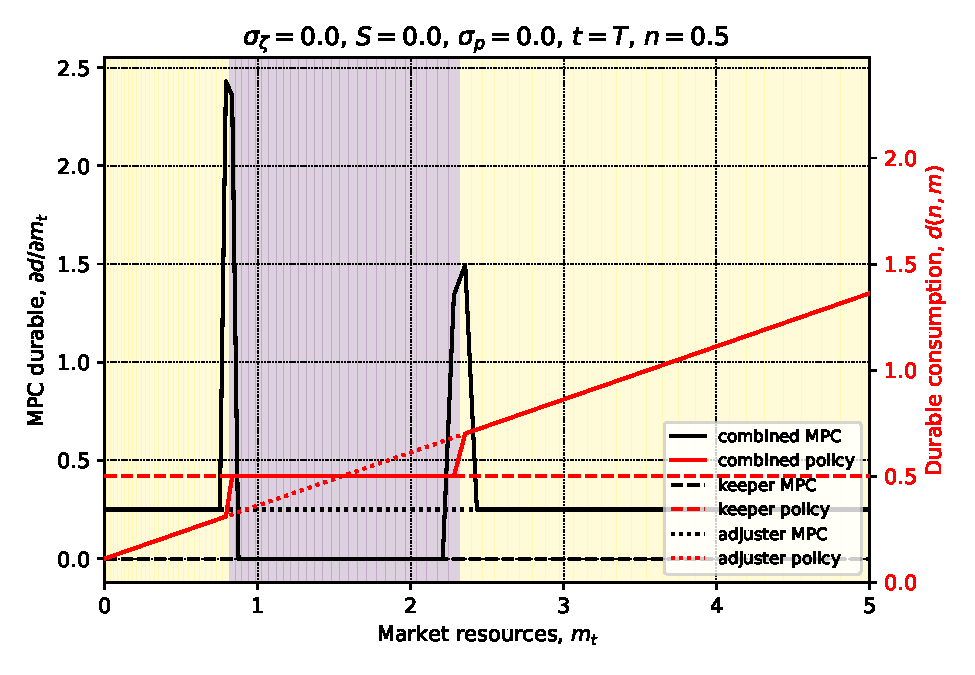
\includegraphics[width=\linewidth]{../Figures/DurableModel/Baseline_d_T_MPC_decomp.pdf}
		\caption{MPC decomposition of durable consumption $d_t(n_t,m_t)$.}
		\label{fig:baseline_d_T_MPC_decomp}
	\end{subfigure}
	\caption{Terminal-period solution of the baseline durable model (hard max). The upper left panel shows the keep--adjust regions in $(m_t,n_t)$ space; the upper right panel shows the combined durable policy for selected beginning-of-period durable stocks $n_t$. The lower panels show the MPC decomposition of nondurable and durable consumption given a fixed beginning-of-period durable stock $n_t$.}
	\label{fig:baseline_T}
\end{figure}
	
	
In earlier periods, the agent incorporates the switchpoints in the next period into the solution of today's problem. Together with non-convex adjustment costs, the first order conditions are only necessary, but not sufficient. Hence, we need to incorporate an upper envelope algorithm such as FUES. However, even with this algorithm, small discontinuities still arise in the adjuster policy functions. Additionally, by combining the keeper and adjuster functions each period, these non-convexities propagade backwards similar to the retirement problem. Figure~\ref{fig:baseline_t_MPC_decomp} illustrates this for a fixed beginning-of-period durable stock $n_t$. In the yellow adjuster region, the policy function and MPC follows the adjuster policy function. With higher market resources, the S,s border gets crossed resulting in stark spikes in MPCs.

\begin{figure}[htbp]
	\centering
	\begin{subfigure}{0.48\textwidth}
		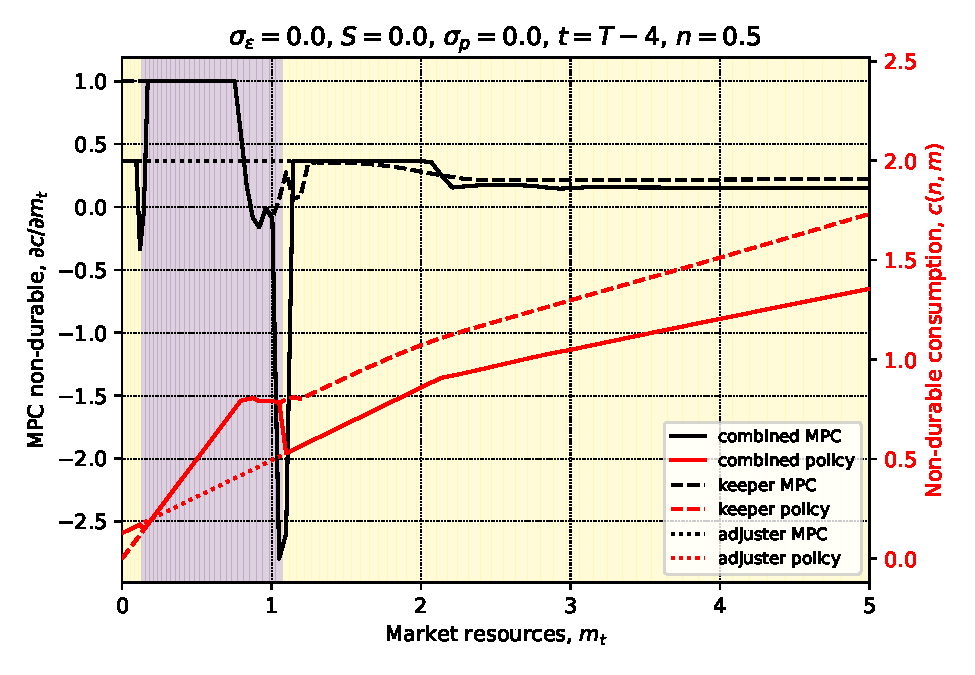
\includegraphics[width=\linewidth]{../Figures/DurableModel/Baseline_c_periodt_MPC_decomp.pdf}
		\caption{MPC decomposition of nondurable consumption $c_t(n_t,m_t)$.}
		\label{fig:baseline_c_periodt_MPC_decomp}
	\end{subfigure}
	\hfill
	\begin{subfigure}{0.48\textwidth}
		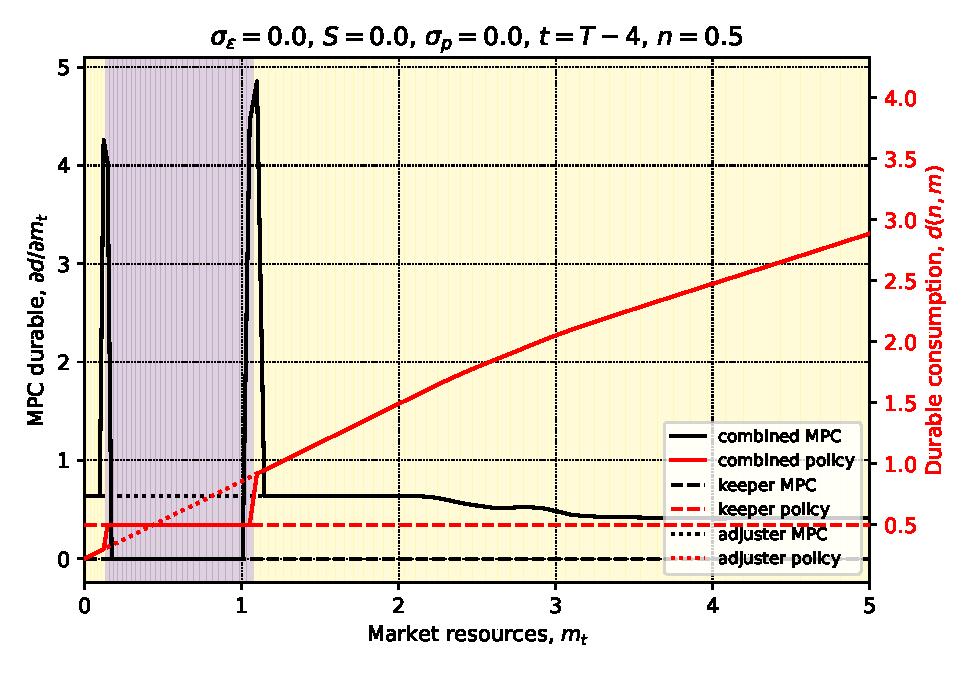
\includegraphics[width=\linewidth]{../Figures/DurableModel/Baseline_d_periodt_MPC_decomp.pdf}
		\caption{MPC decomposition of durable consumption $d_t(n_t,m_t)$.}
		\label{fig:baseline_d_periodt_MPC_decomp}
	\end{subfigure}
	\caption{MPC and policy functions of non-durable and durable consumption.}
	\label{fig:baseline_t_MPC_decomp}
\end{figure}
\subsection{Extension: Extreme Value Type I Taste Shocks}\label{subsec:ModelBasicTaste}

The hard maximum in the discrete keep-versus-adjust decision produces a kink in the value function and a discontinuity in the policy functions at the state combinations $(m_t,n_t)$ where the household is indifferent between the two branches. Following the discrete--continuous choice literature (e.g.\ \cite{Iskhakov2017-jb}), this subsection smooths that discontinuity with i.i.d.\ Extreme Value Type I (Gumbel) taste shocks on the two discrete alternatives, while leaving search frictions aside (these are introduced separately in Section~\ref{subsec:ModelBasicSearch}). Unlike the multiplicative mean-one log-normal taste shocks used in the retirement application of Section~\ref{sec:RetirementModel}, EV Type I shocks enter \emph{additively} on each branch and are integrated out in closed form: they randomize the discrete outcome directly through logit choice probabilities, without introducing an additional continuous (or discretized) state.

At the start of period $t$, after observing $(m_t,n_t)$, the household draws i.i.d.\ Extreme Value Type I shocks $(\varepsilon_t^{\text{keep}},\varepsilon_t^{\text{adj}})$ and chooses the branch that maximizes the shock-augmented conditional value,
\begin{align}
	v_t(m_t,n_t)
	&= \max\Big\{
		v_t^{\text{keep}}(m_t,n_t) + \sigma_\varepsilon\,\varepsilon_t^{\text{keep}},\;
		v_t^{\text{adj}}(\ell_t) + \sigma_\varepsilon\,\varepsilon_t^{\text{adj}}
	\Big\}, \label{eq:taste_discrete_EV}
\end{align}
where $\sigma_\varepsilon > 0$ is the taste-shock scale and $\ell_t = m_t+(1-\tau)n_t$. The conditional value functions $v_t^{\text{keep}}(m_t,n_t)$ and $v_t^{\text{adj}}(\ell_t)$ retain exactly the same Bellman definitions as in the baseline model: the taste shocks do not enter the inner continuous maximizations, so the first-order conditions~\eqref{eq:FOC_c_basic}--\eqref{eq:FOC_d_basic} and the continuous policies $c_t^{\text{keep}}$, $c_t^{\text{adj}}$, $d_t^{\text{adj}}$ are unchanged.

Because $(\varepsilon_t^{\text{keep}},\varepsilon_t^{\text{adj}})$ are i.i.d.\ Extreme Value Type I, the expectation of~\eqref{eq:taste_discrete_EV} has the closed-form log-sum representation
\begin{align}
	v_t(m_t,n_t)
	&= \sigma_\varepsilon \log\Big(
		\exp\big(v_t^{\text{keep}}(m_t,n_t)/\sigma_\varepsilon\big)
		+ \exp\big(v_t^{\text{adj}}(\ell_t)/\sigma_\varepsilon\big)
	\Big), \label{eq:taste_logsum}
\end{align}
with logit choice probabilities
\begin{align}
	P_t^{\text{adj}}(m_t,n_t)
	&= \frac{\exp\big(v_t^{\text{adj}}(\ell_t)/\sigma_\varepsilon\big)}
	{\exp\big(v_t^{\text{keep}}(m_t,n_t)/\sigma_\varepsilon\big)
	+ \exp\big(v_t^{\text{adj}}(\ell_t)/\sigma_\varepsilon\big)},
	\qquad
	P_t^{\text{keep}}(m_t,n_t) = 1 - P_t^{\text{adj}}(m_t,n_t). \label{eq:taste_logit}
\end{align}
The expected (ex-ante) policy functions are the probability-weighted averages of the two branches,
\begin{align}
	c_t(m_t,n_t) &= P_t^{\text{keep}}\, c_t^{\text{keep}}(m_t,n_t) + P_t^{\text{adj}}\, c_t^{\text{adj}}(\ell_t), \label{eq:taste_c_combined}\\
	d_t(m_t,n_t) &= P_t^{\text{keep}}\, n_t + P_t^{\text{adj}}\, d_t^{\text{adj}}(\ell_t). \label{eq:taste_d_combined}
\end{align}
As $\sigma_\varepsilon \to 0$, the logit probabilities collapse to the hard indicators of the baseline model and~\eqref{eq:taste_logsum} collapses to the hard maximum. Larger $\sigma_\varepsilon$ spreads probability mass onto the inferior branch near indifference, so $c_t$ and $d_t$ (and the marginal-value functions derived from the inclusive value~\eqref{eq:taste_logsum}) are smooth in $(m_t,n_t)$. No quadrature over taste nodes is required: the EV Type I assumption delivers the inclusive value and choice probabilities in closed form. The taste shocks do not alter the household's budget set, so the no-borrowing constraint $a_t \ge 0$ is unaffected. I derive the envelope conditions, the Euler equations, and the EGM algorithm with EV Type I taste shocks in appendix~\ref{subsec:appdx_taste_basic}.

As a result, the S,s curve in the terminal period is smoothened and adjuster values between zero and one are optimal. In the aggregate, the policy functions are a convex combination of adjuster and keeper policy functions around the S,s thresholds. Fig~\ref{fig:tasteshock_T} illustrates the point clearly.

\begin{figure}[htbp]
	\centering
	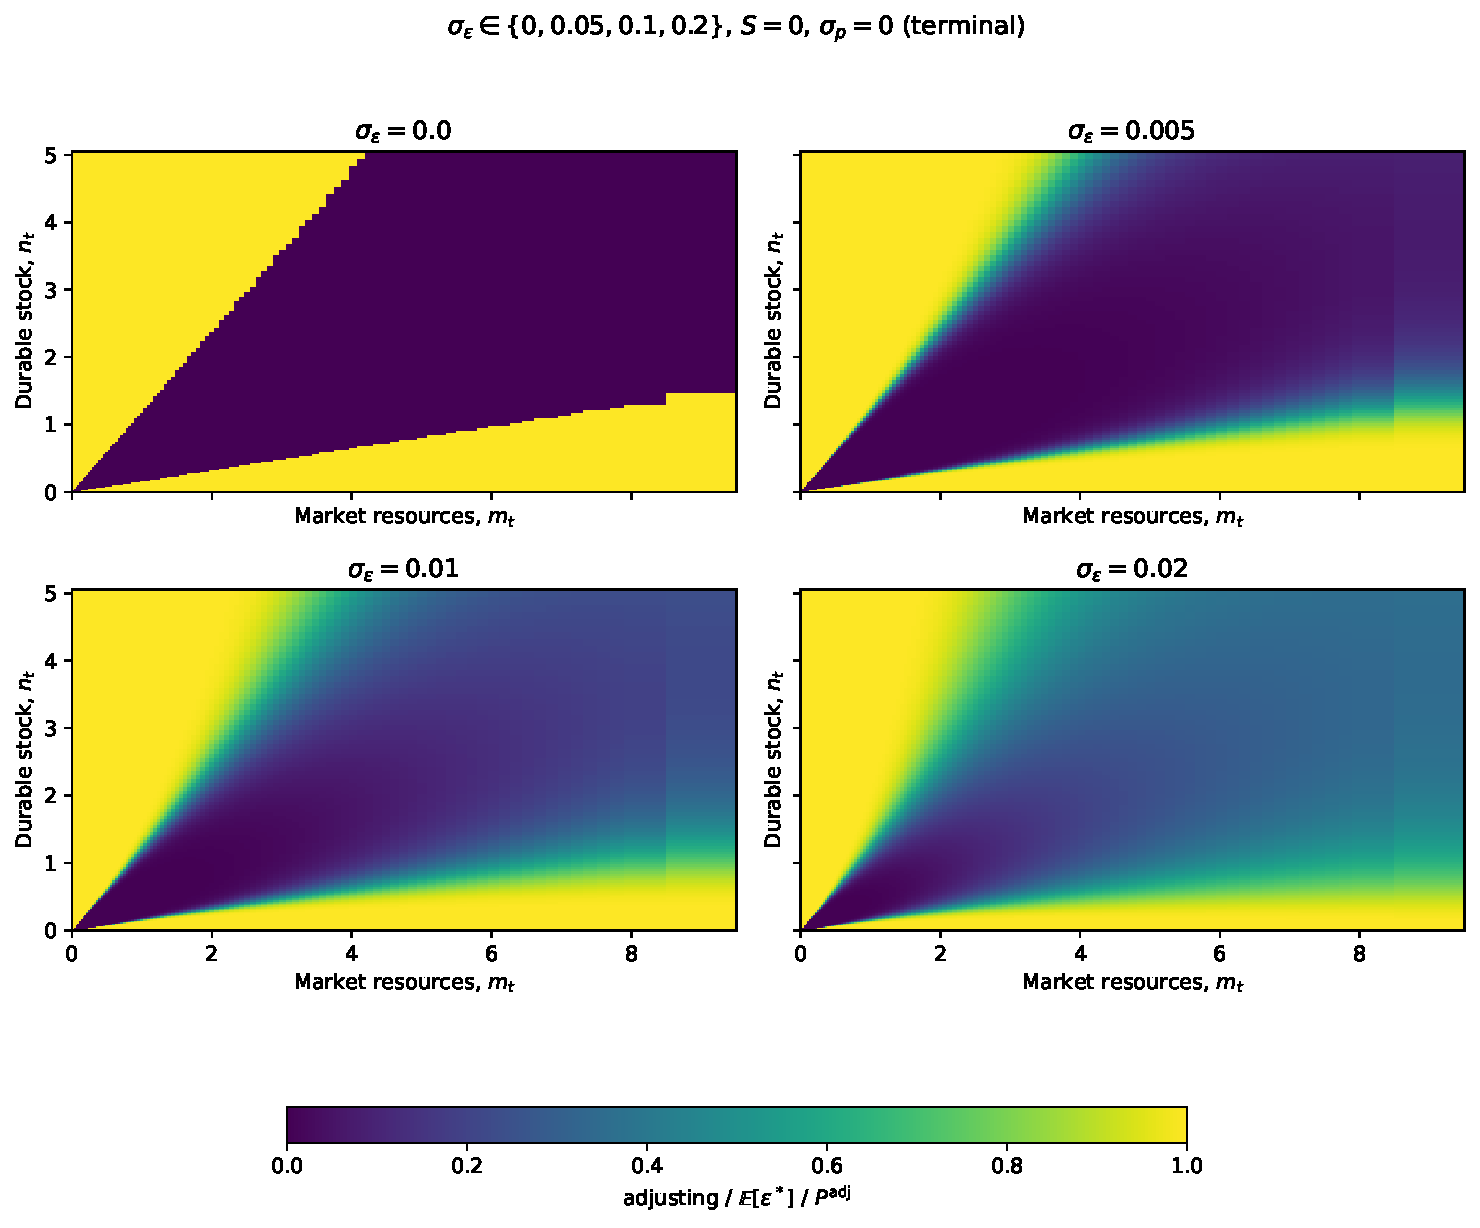
\includegraphics[width=\linewidth]{../Figures/DurableModel/TasteShock_Ss_T.pdf}
	\caption{Terminal-period keep--adjust regions in $(m_t,n_t)$ space under EV Type I taste shocks for $\sigma_\varepsilon \in \{0, 0.05, 0.1, 0.2\}$.}
	\label{fig:tasteshock_ss_T}
	\label{fig:tasteshock_T}
\end{figure}

As a result, the discontinuities in period t disapear with a small EV shock parameter. Fig~\ref{fig:tasteshock_periodt_MPC_decomp} show the now continuous consumption functions and marginal propensities to consume and expend.


\begin{figure}[htbp]
	\centering
	\begin{subfigure}{0.48\textwidth}
		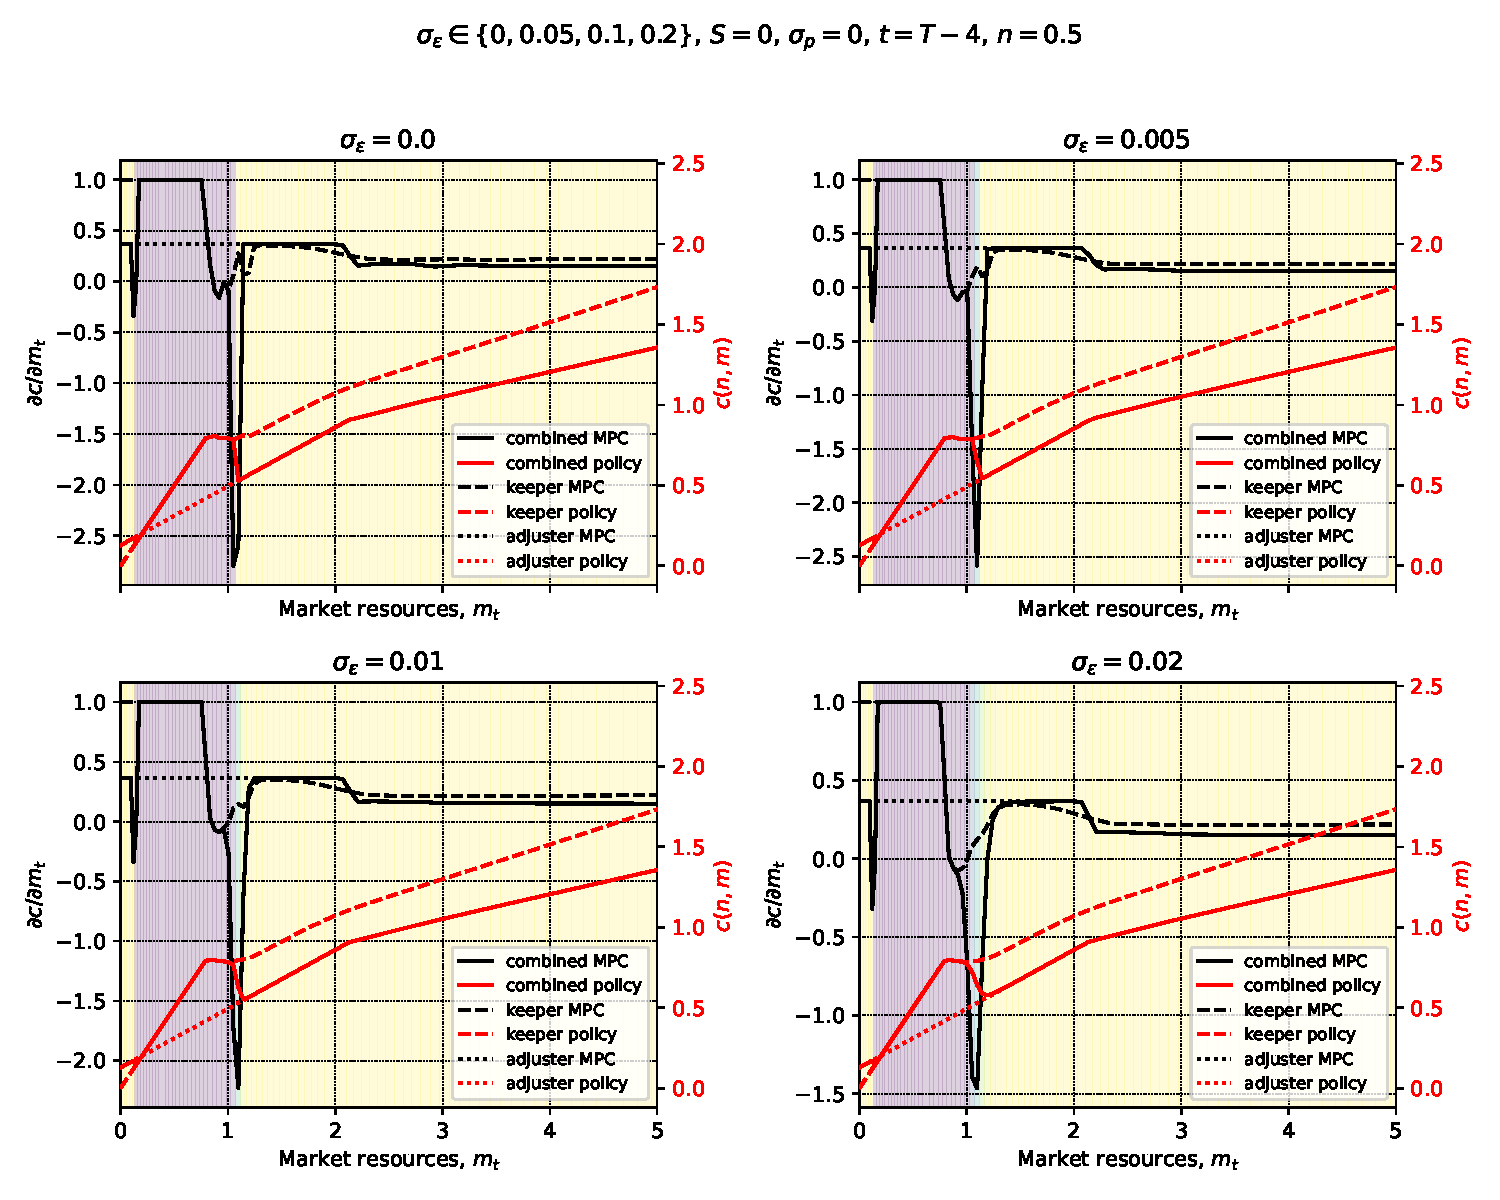
\includegraphics[width=\linewidth]{../Figures/DurableModel/TasteShock_c_periodt_MPC_decomp.pdf}
		\caption{MPC decomposition of nondurable consumption $c_t(n_t,m_t)$.}
		\label{fig:tasteshock_c_periodt_MPC_decomp}
	\end{subfigure}
	\hfill
	\begin{subfigure}{0.48\textwidth}
		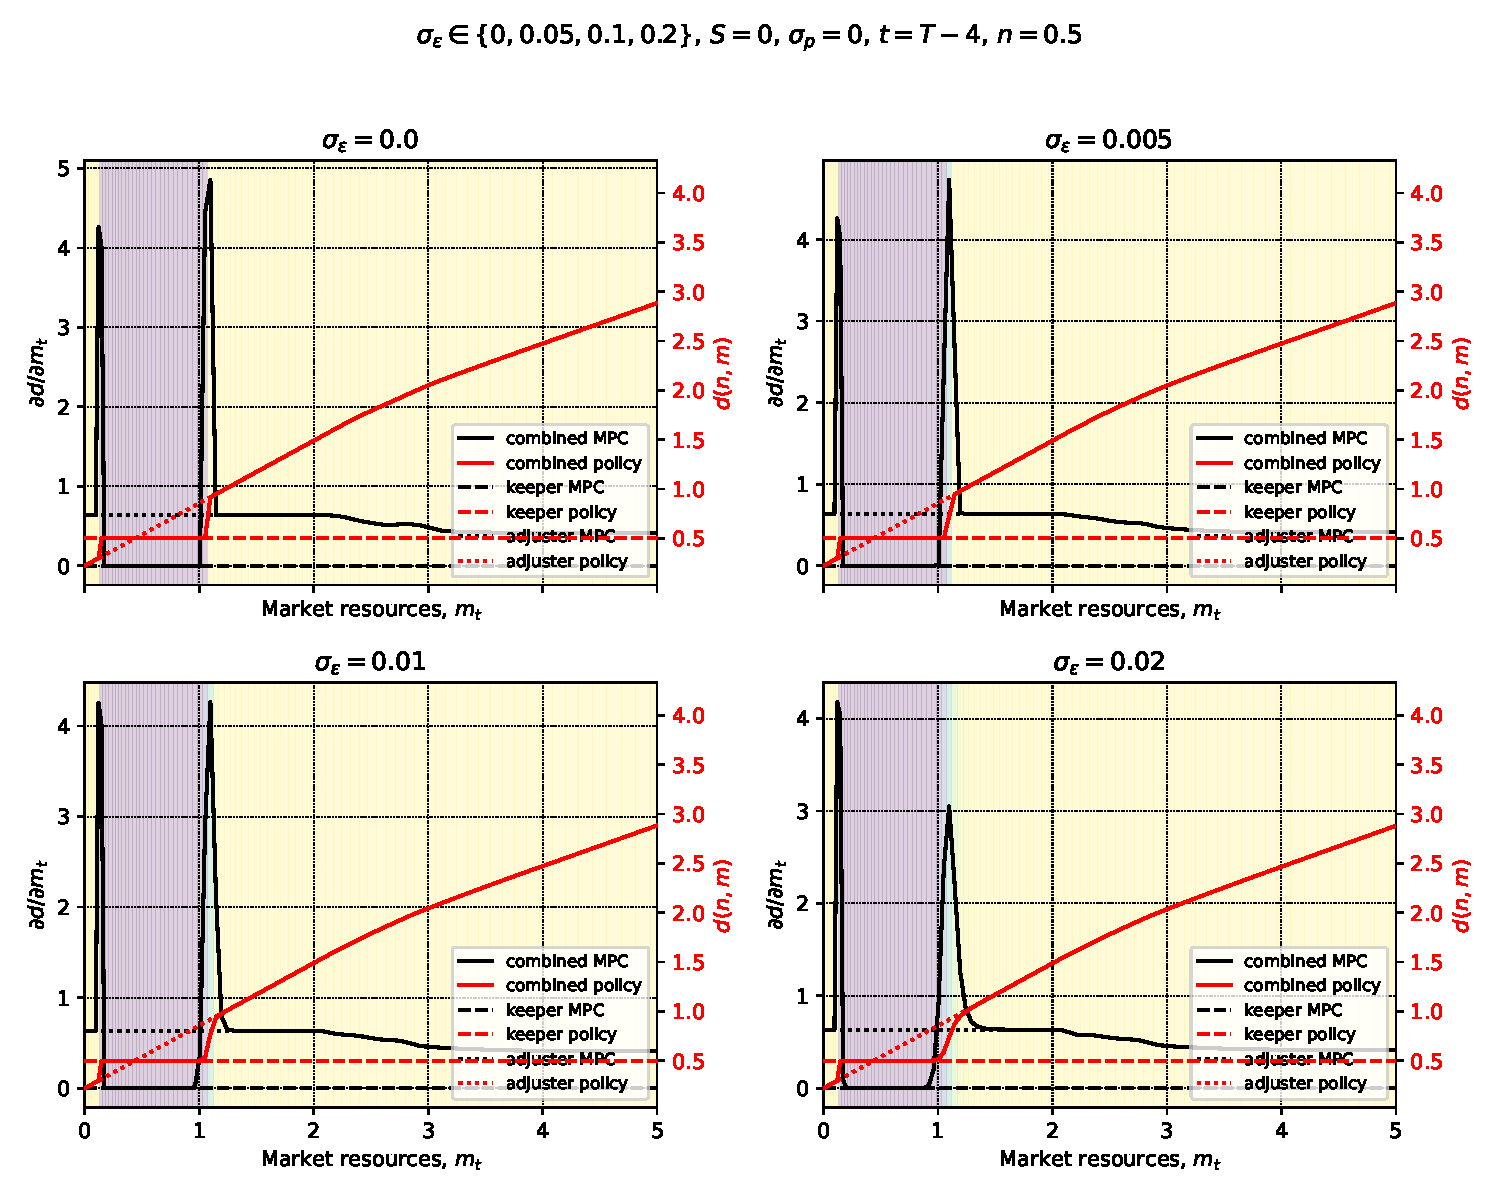
\includegraphics[width=\linewidth]{../Figures/DurableModel/TasteShock_d_periodt_MPC_decomp.pdf}
		\caption{MPC decomposition of durable consumption $d_t(n_t,m_t)$.}
		\label{fig:tasteshock_d_periodt_MPC_decomp}
	\end{subfigure}
	\caption{MPC and policy functions of non-durable and durable consumption using EV taste shocks.}
	\label{fig:tasteshock_periodt_MPC_decomp}
\end{figure}

\subsection{Extension: Search Frictions}\label{subsec:ModelBasicSearch}

This subsection instead reintroduces the directed-search mechanism of the full model into the basic environment, without taste shocks. Rather than resolving the keep-versus-adjust margin with a hard maximum, the household chooses a search intensity $\varepsilon_t \in [0,1]$ that determines the weight placed on the adjuster's conditional value in the current period. Exerting search effort is costly, with cost function
\begin{align}
	\sigma(\varepsilon_t) = S\big[\varepsilon_t + (1-\varepsilon_t)\log(1-\varepsilon_t)\big], \label{eq:search_cost_basic}
\end{align}
where $S>0$ governs the degree of friction in the market for durables, following \cite{Khan2019-ew}. The beginning-of-period problem becomes
\begin{align}
	v_t(m_t,n_t) = \max_{\varepsilon_t \in [0,1]} \Big[(1-\varepsilon_t)\, v_t^{\text{keep}}(m_t,n_t) + \varepsilon_t\, v_t^{\text{adj}}(\ell_t) - \sigma(\varepsilon_t)\Big], \label{eq:search_discrete_basic}
\end{align}
where $v_t^{\text{keep}}$ and $v_t^{\text{adj}}$ retain exactly the same Bellman definitions as in the baseline model, except that the continuation value $v_{t+1}(m_{t+1},n_{t+1})$ appearing inside them is now itself given recursively by equation~\eqref{eq:search_discrete_basic} one period ahead, rather than by the hard maximum of the baseline model. All other features of the basic environment---the single interest rate $\mathcal{R}$, the absence of maintenance costs, and the no-borrowing constraint $a_t \ge 0$---are unchanged.

Search effort is chosen before the discrete outcome is known: $\varepsilon_t$ can be interpreted as the probability with which the household successfully locates a suitable durable this period, so the combined value function~\eqref{eq:search_discrete_basic} is a probability-weighted average of the two conditional values, net of the search cost. As $S \to 0$, search becomes costless, the household sets $\varepsilon_t \in \{0,1\}$, and the model collapses to the hard-maximum baseline; as $S \to \infty$, search becomes prohibitively costly, $\varepsilon_t^\ast \to 0$, and the household never adjusts. I derive the optimal search-effort rule, the smooth combined marginal-value functions, and the associated EGM steps in appendix~\ref{subsec:appdx_search_basic}.

Endogeneous search achieves a similar smoothing compared to the EV shocks. Fig~\ref{fig:search_ss_T} illustrates the terminal period solution. A small search cost is sufficient to lead to a smoothened S,s region.

\begin{figure}[htbp]
	\centering
	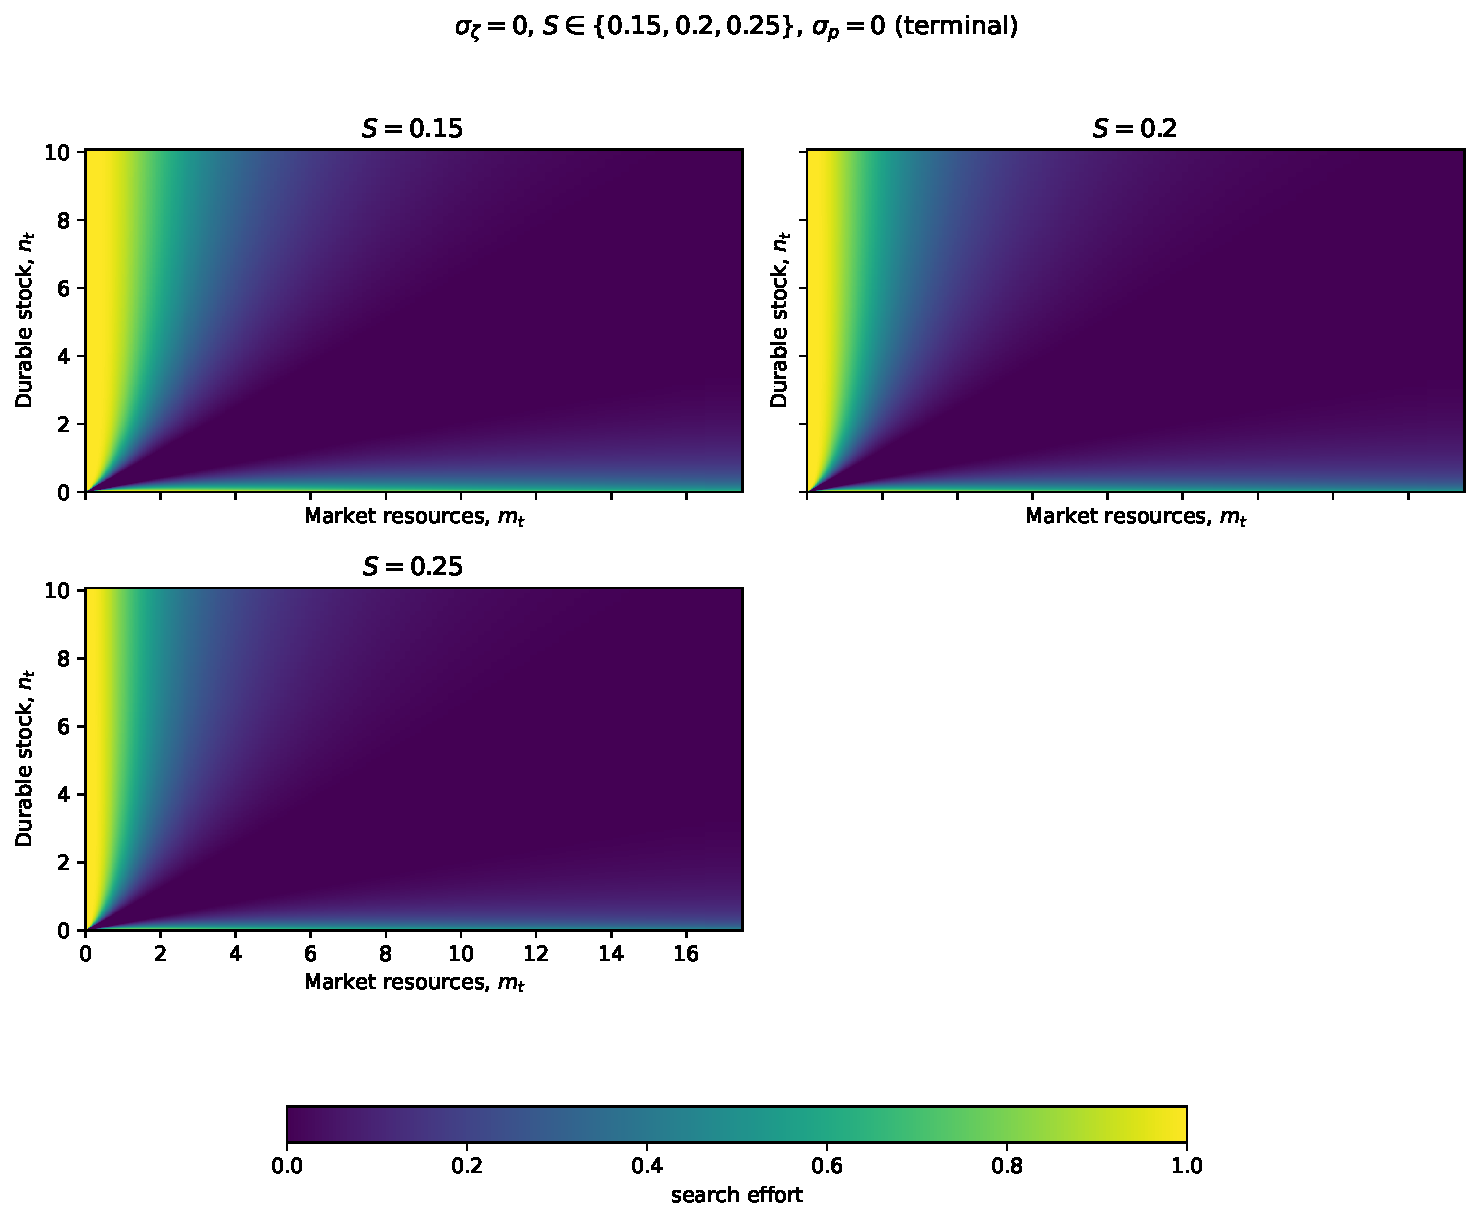
\includegraphics[width=\linewidth]{../Figures/DurableModel/Search_Ss_T.pdf}
	\caption{Terminal-period keep--adjust regions in $(m_t,n_t)$ space under endogeneous search for search-cost scales $S \in \{0, 0.05, 0.1, 0.2\}$.}
	\label{fig:search_ss_T}
\end{figure}

As a result, optimal consumption functions in period t are smooth as well (see fig~\ref{fig:search_periodt_MPC_decomp}).

\begin{figure}[htbp]
	\centering
	\begin{subfigure}{0.48\textwidth}
		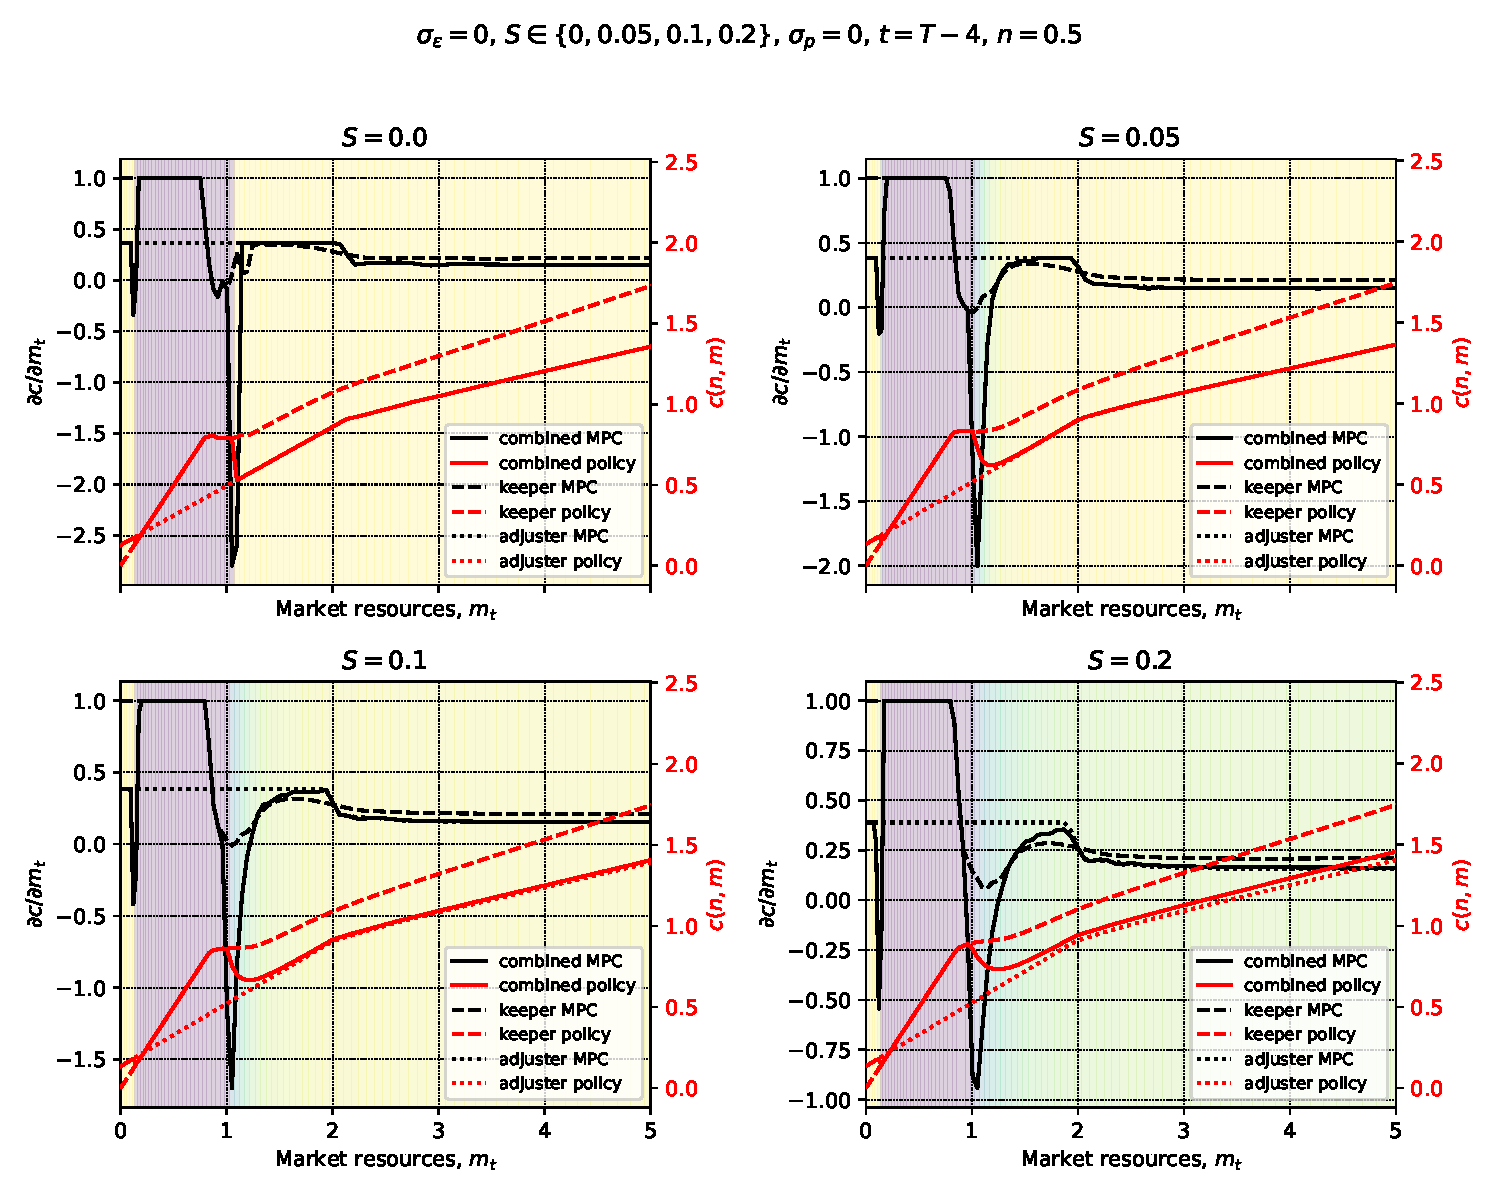
\includegraphics[width=\linewidth]{../Figures/DurableModel/Search_c_periodt_MPC_decomp.pdf}
		\caption{MPC decomposition of nondurable consumption $c_t(n_t,m_t)$.}
		\label{fig:search_c_periodt_MPC_decomp}
	\end{subfigure}
	\hfill
	\begin{subfigure}{0.48\textwidth}
		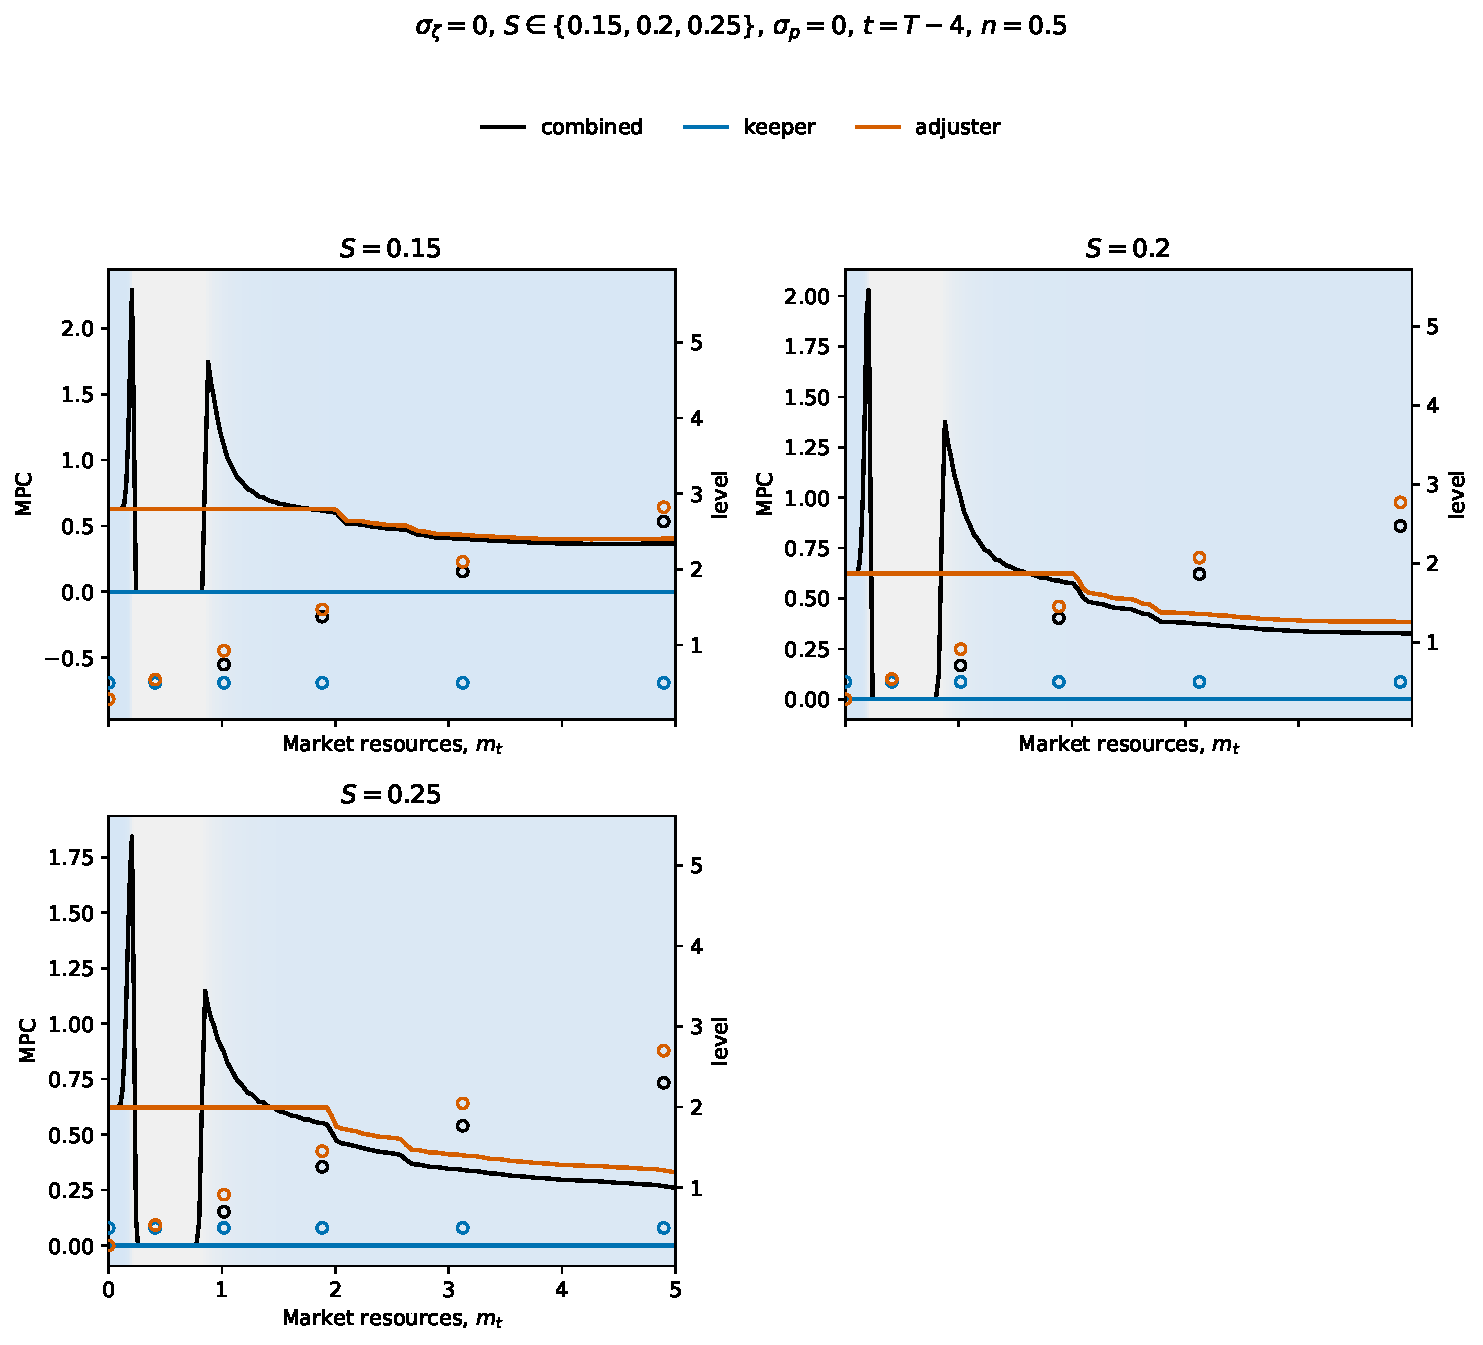
\includegraphics[width=\linewidth]{../Figures/DurableModel/Search_d_periodt_MPC_decomp.pdf}
		\caption{MPC decomposition of durable consumption $d_t(n_t,m_t)$.}
		\label{fig:search_d_periodt_MPC_decomp}
	\end{subfigure}
	\caption{MPC and policy functions of non-durable and durable consumption using endogeneous search.}
	\label{fig:search_periodt_MPC_decomp}
\end{figure}


\subsection{Extension: Stochastic Durable Prices}\label{subsec:ModelBasicPrice}

This subsection introduces a third source of variation, orthogonal to the taste shocks of Section~\ref{subsec:ModelBasicTaste} and the search frictions of Section~\ref{subsec:ModelBasicSearch}: an idiosyncratic, i.i.d.\ shock to the relative price at which the durable good can be purchased in the period of adjustment. Neither taste shocks nor search frictions are present in this subsection, so the discrete choice between keeping and adjusting again resolves through a hard maximum, but now the adjuster's problem---and hence the comparison itself---is contingent on the realized price.

At the start of period $t$, after the transitory income shock $\theta_t$ has materialized, the household observes an i.i.d.\ relative price $p_t$ at which new units of the durable good can be bought this period. The price is log-normally distributed with mean one,
\begin{align}
	\log p_t \sim \mathcal{N}\Big(-\frac{\sigma_p^2}{2},\, \sigma_p^2\Big), \qquad \mathbb{E}[p_t] = 1, \label{eq:price_dist}
\end{align}
independent of $\theta_t$ and independent across periods. Only the \emph{purchase} of new durables is exposed to this price risk: households liquidate their existing durable stock exactly as in the baseline model, at the fixed proportional recovery rate $1-\tau$, so the liquidity available upon adjustment, $\ell_t = m_t + (1-\tau)n_t$, is unaffected by $p_t$. This is consistent with an interpretation in which trading in a used durable is governed by a separate, deterministic adjustment cost, while the price of a new unit on the market this period fluctuates, e.g.\ a household trading in a used car against the fluctuating price of a new one.

The keeper's problem is entirely unaffected by $p_t$, since no purchase occurs, so $v_t^{\text{keep}}(m_t,n_t)$ retains its baseline Bellman definition. The adjuster's budget constraint, however, now reads
\begin{align}
	a_t = \ell_t - c_t - p_t\, d_t \ge 0, \label{eq:price_budget}
\end{align}
in place of $a_t=\ell_t-c_t-d_t$, so the conditional value function becomes a function of both $\ell_t$ and $p_t$,
\begin{align}
	v_t^{\text{adj}}(\ell_t,p_t) &= \max_{c_t,d_t} \ u(c_t,d_t) + \beta \mathbb{E}_t \big[ v_{t+1}(m_{t+1},n_{t+1}) \big],\\
	& \text{s.t. equation~\eqref{eq:price_budget},}\\
	& \qquad m_{t+1} = \mathcal{R} a_t + \theta_{t+1}, \qquad n_{t+1} = (1-\delta)\,d_t.
\end{align}
Everything else about the household's environment---the interest rate $\mathcal{R}$, the depreciation rate $\delta$, and the no-borrowing constraint $a_t \ge 0$---is unchanged, and next period's durable stock $n_{t+1}$ continues to be measured in physical units, so $p_t$ affects only the current-period cost of acquiring $d_t$, not its future service flow beyond ordinary depreciation.

With the price-contingent budget constraint~\eqref{eq:price_budget}, the adjuster's Lagrangian is
\begin{align}
	\mathscr{L} = u(c_t,d_t) + \beta \mathbb{E}_t\big[v_{t+1}(m_{t+1},n_{t+1})\big] + \lambda_t^{\mathrm{adj}}\big(\ell_t - c_t - p_t\, d_t - a_t\big),
\end{align}
with $m_{t+1}=\mathcal{R}a_t+\theta_{t+1}$ and $n_{t+1}=(1-\delta)d_t$. The first-order conditions with respect to $c_t$, $a_t$, and $d_t$ are
\begin{align}
	\frac{\partial \mathscr{L}}{\partial c_t} &= u_c(c_t,d_t) - \lambda_t^{\mathrm{adj}} = 0
	&&\Longrightarrow\quad \lambda_t^{\mathrm{adj}} = u_c(c_t,d_t), \label{eq:price_foc_c}\\
	\frac{\partial \mathscr{L}}{\partial a_t} &= \beta \mathcal{R}\, \mathbb{E}_t\big[v_{t+1}^m\big] - \lambda_t^{\mathrm{adj}} = 0
	&&\Longrightarrow\quad \lambda_t^{\mathrm{adj}} = \beta \mathcal{R}\, \mathbb{E}_t\big[v_{t+1}^m\big], \label{eq:price_foc_a}\\
	\frac{\partial \mathscr{L}}{\partial d_t} &= u_d(c_t,d_t) + \beta(1-\delta)\,\mathbb{E}_t\big[v_{t+1}^n\big] - p_t\,\lambda_t^{\mathrm{adj}} = 0
	&&\Longrightarrow\quad u_d(c_t,d_t) = p_t\,\lambda_t^{\mathrm{adj}} - \beta(1-\delta)\,\mathbb{E}_t\big[v_{t+1}^n\big]. \label{eq:price_foc_d}
\end{align}
In KKT form, these are the price-modified analogues of the baseline conditions~\eqref{eq:FOC_c_basic}--\eqref{eq:FOC_d_basic}:
\begin{align}
	u_c(c_t, d_t) &\geq \beta \mathcal{R}\, \mathbb{E}_t \big[v_{t+1}^m\big], \\
	u_d(c_t, d_t) &\geq p_t\,\beta \mathcal{R}\, \mathbb{E}_t\big[v_{t+1}^m\big] - \beta (1 - \delta)\, \mathbb{E}_t\big[v_{t+1}^n\big].
\end{align}
Equation~\eqref{eq:price_foc_c} is identical in form to~\eqref{eq:FOC_c_basic}: because $p_t$ multiplies only $d_t$ in the budget, it does not appear in the $c_t$ first-order condition, so $c_t^{\mathrm{adj},\ast}$ solves the same equation as in the baseline model \emph{given} $d_t$. Equation~\eqref{eq:price_foc_d} differs from~\eqref{eq:FOC_d_basic}: the marginal cost of an extra unit of durables is now $p_t\lambda_t^{\mathrm{adj}}$ rather than $\lambda_t^{\mathrm{adj}}$, since each unit of $d_t$ costs $p_t$ units of $\ell_t$ instead of one. Equality holds when the borrowing constraint does not bind.

Because $p_t$ is observed before the discrete choice is made, the household's beginning-of-period problem is the price-contingent hard maximum
\begin{align}
	v_t(m_t,n_t,p_t) = \max\Big\{ v_t^{\text{keep}}(m_t,n_t),\; v_t^{\text{adj}}(\ell_t,p_t)\Big\}. \label{eq:price_discrete}
\end{align}
A high realization of $p_t$ raises the marginal cost of adjusting and, other things equal, makes the household less likely to adjust and, conditional on adjusting, to purchase a smaller quantity of the durable; a low realization has the opposite effect. Because agents can reject an offer when the drawn price leads to an allocation which is worse than the keeper solution, the model induces state-contingent variation in both the adjustment margin and the size of the resulting durable purchase.

As with the EV Type I inclusive value, the object that matters for the previous period's continuation value is the price-integrated value function
\begin{align}
	\bar v_t(m_t,n_t) \equiv \mathbb{E}_{p_t}\Big[v_t(m_t,n_t,p_t)\Big]
	= \mathbb{E}_{p_t}\Big[\max\big\{ v_t^{\text{keep}}(m_t,n_t),\; v_t^{\text{adj}}(\ell_t,p_t) \big\}\Big], \label{eq:price_barv}
\end{align}
which replaces $v_t(m_t,n_t)$ inside the Bellman equations for $v_{t-1}^{\text{keep}}$ and $v_{t-1}^{\text{adj}}$. Unlike EV Type I taste shocks, which leave the adjuster's optimal continuous choices unchanged and only reweight the discrete comparison through logit probabilities, the price shock changes the adjuster's optimal consumption-durable split itself, so $v_t^{\text{adj}}(\ell_t,p_t)$ must be solved separately for every relevant realization of $p_t$; the resulting policy functions $c_t^{\text{adj}}(\ell_t,p_t)$ and $d_t^{\text{adj}}(\ell_t,p_t)$ are likewise price-contingent, and the model's reported (ex-ante) nondurable-consumption and durable-purchase functions are price-weighted averages of these state-contingent choices, in the same spirit as $\bar v_t$. As $\sigma_p \to 0$, $p_t \to 1$ almost surely and the model collapses to the hard-maximum baseline of Section~\ref{sec:ModelBasic}. I derive the envelope conditions, the terminal-period solution, and the EGM algorithm with stochastic durable prices in appendix~\ref{subsec:appdx_price_basic}.

Even stochastic prices induce enough uncertainty to lead to adjusting intensities between zero and one as seen in
fig~\ref{fig:pricestd_Ss_T}. However, since sharp thresholds still exist, the consumption functions in T-1 are not as smooth as with taste shocks or endogeneous search.

\begin{figure}[htbp]
	\centering
	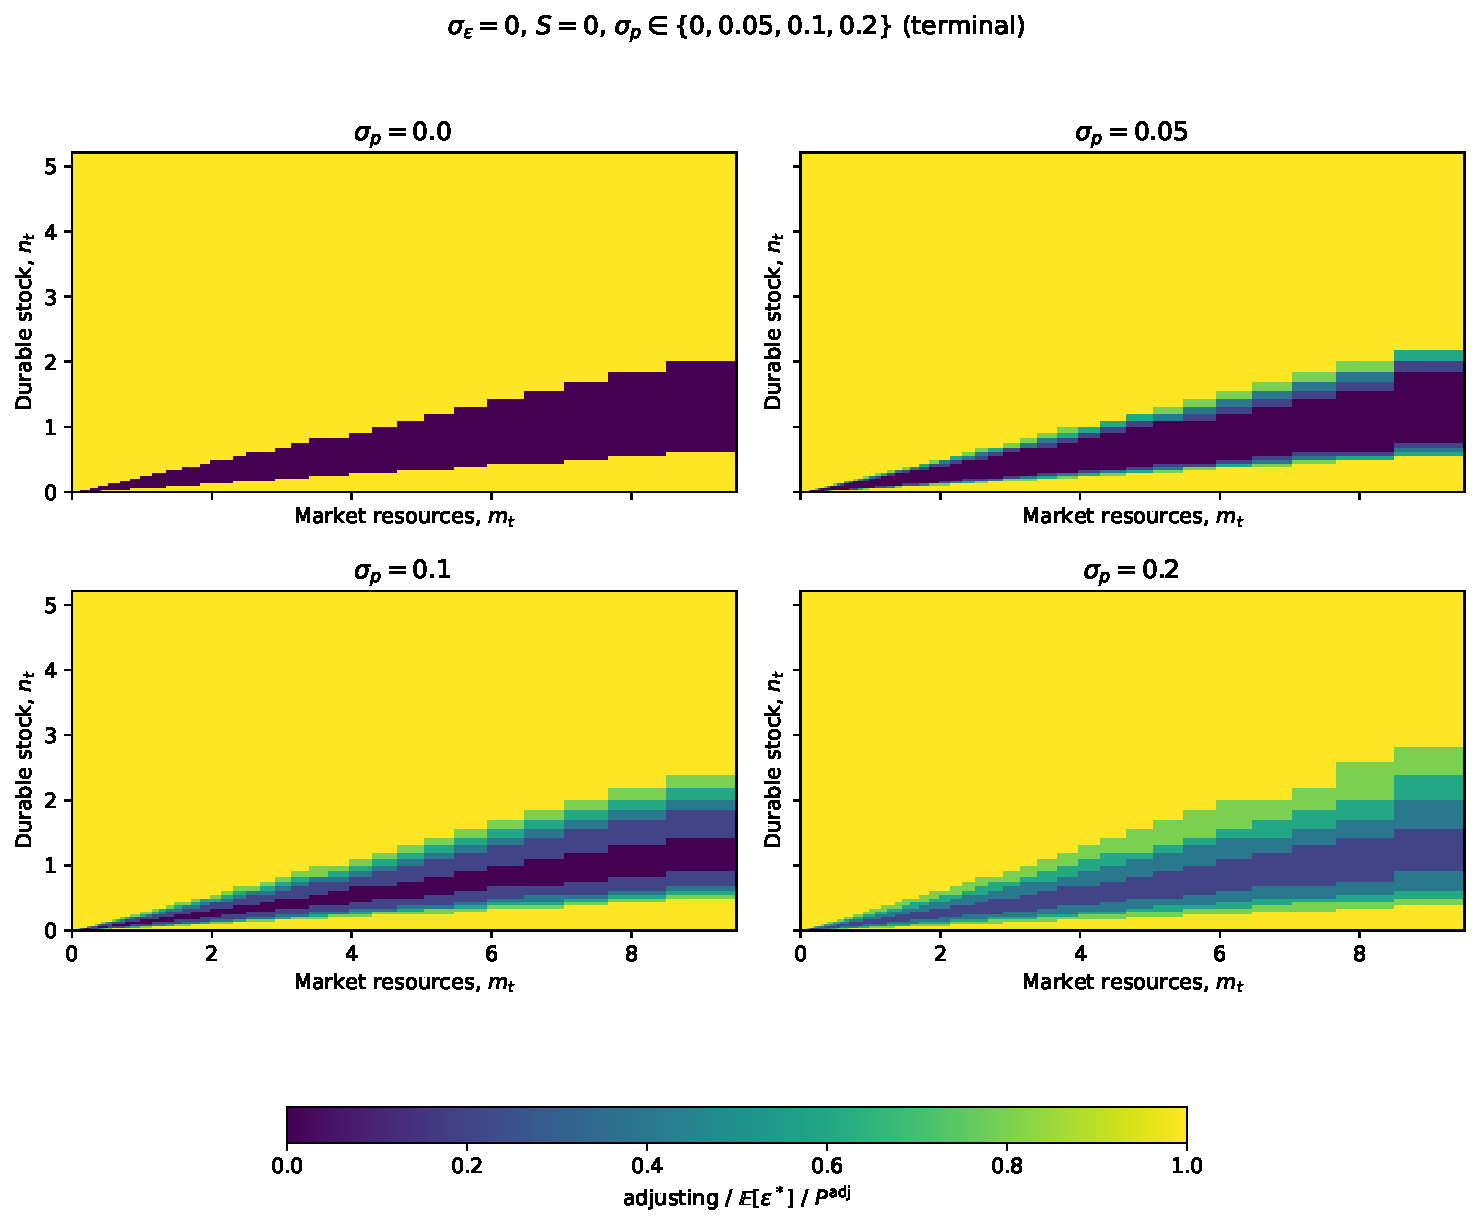
\includegraphics[width=0.85\linewidth]{../Figures/DurableModel/PriceStd_Ss_T.pdf}
	\caption{Adjustment regions in period $T$ under stochastic durable prices for $\sigma_p \in \{0, 0.05, 0.1, 0.2\}$ (fixed number of price nodes). Greater price dispersion softens the hard keep--adjust threshold.}
	\label{fig:pricestd_Ss_T}
\end{figure}

Figure~\ref{fig:PriceStd_periodt_MPC_decomp} shows the policy functions for variation in the price dispersion and figure~\ref{fig:PriceCount_periodt_MPC_decomp} for a coraser grid of price points.

\begin{figure}[htbp]
	\centering
	\begin{subfigure}{0.48\textwidth}
		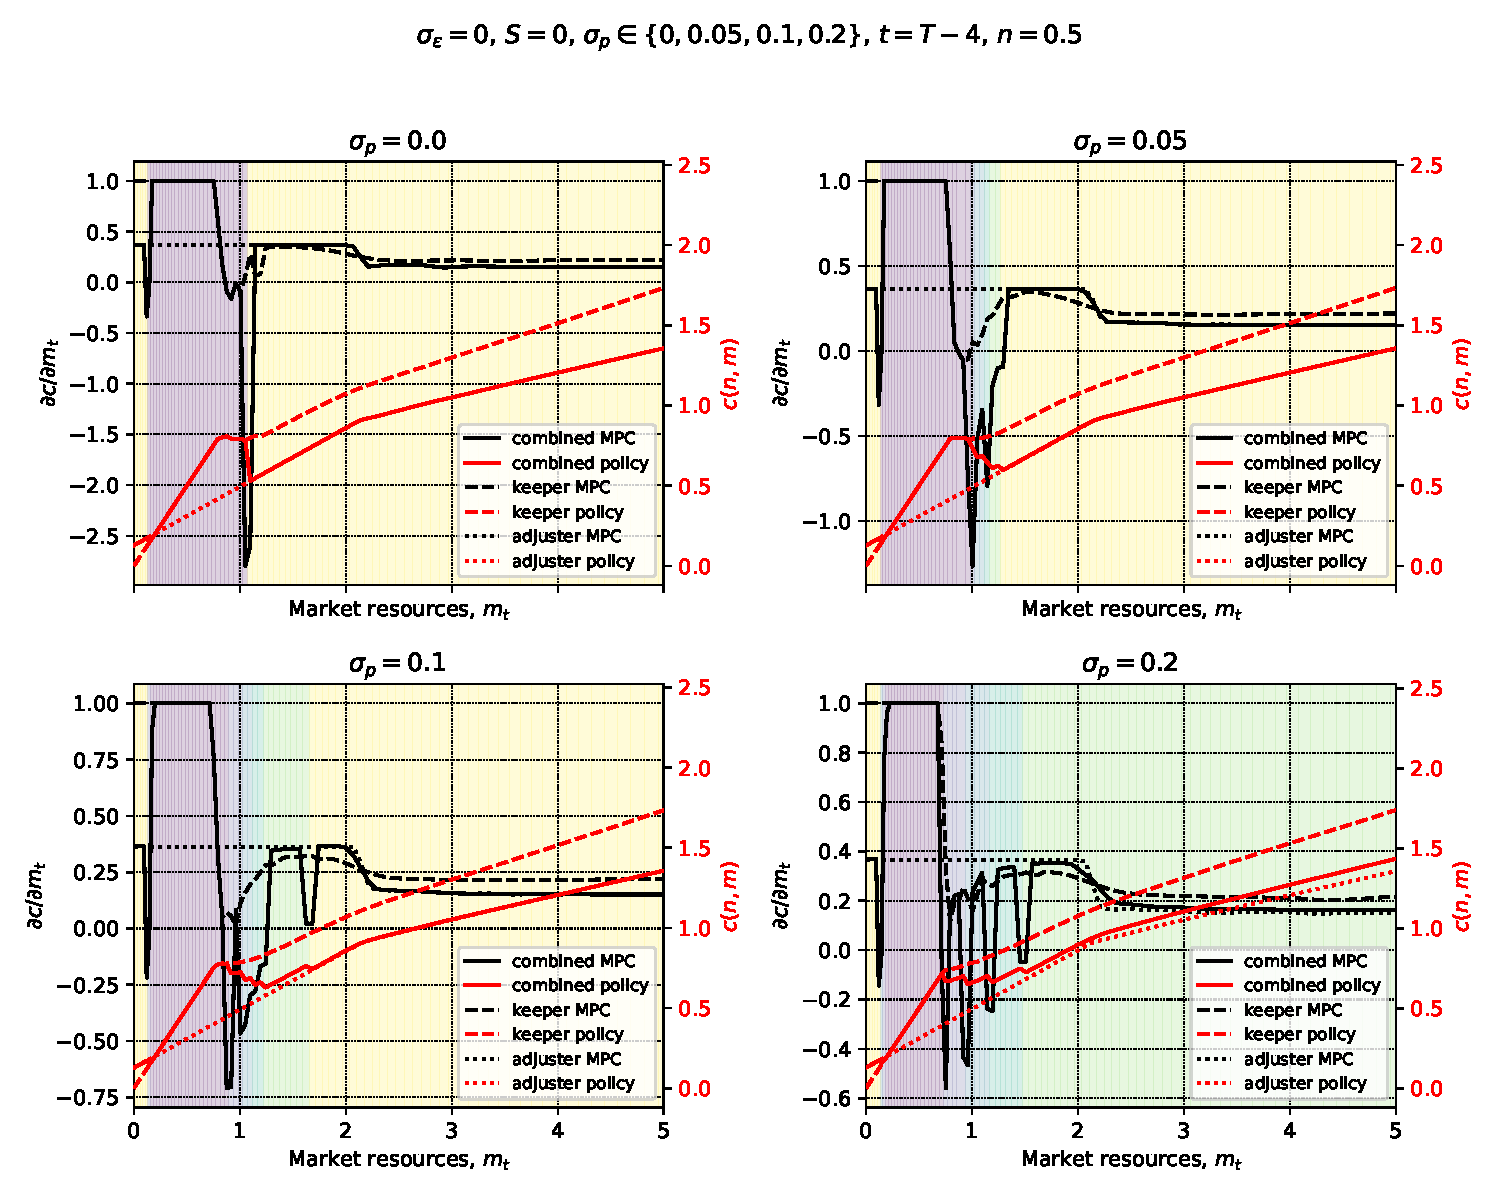
\includegraphics[width=\linewidth]{../Figures/DurableModel/PriceStd_c_periodt_MPC_decomp.pdf}
		\caption{MPC decomposition of nondurable consumption $c_t(n_t,m_t)$.}
		\label{fig:PriceStd_c_periodt_MPC_decomp}
	\end{subfigure}
	\hfill
	\begin{subfigure}{0.48\textwidth}
		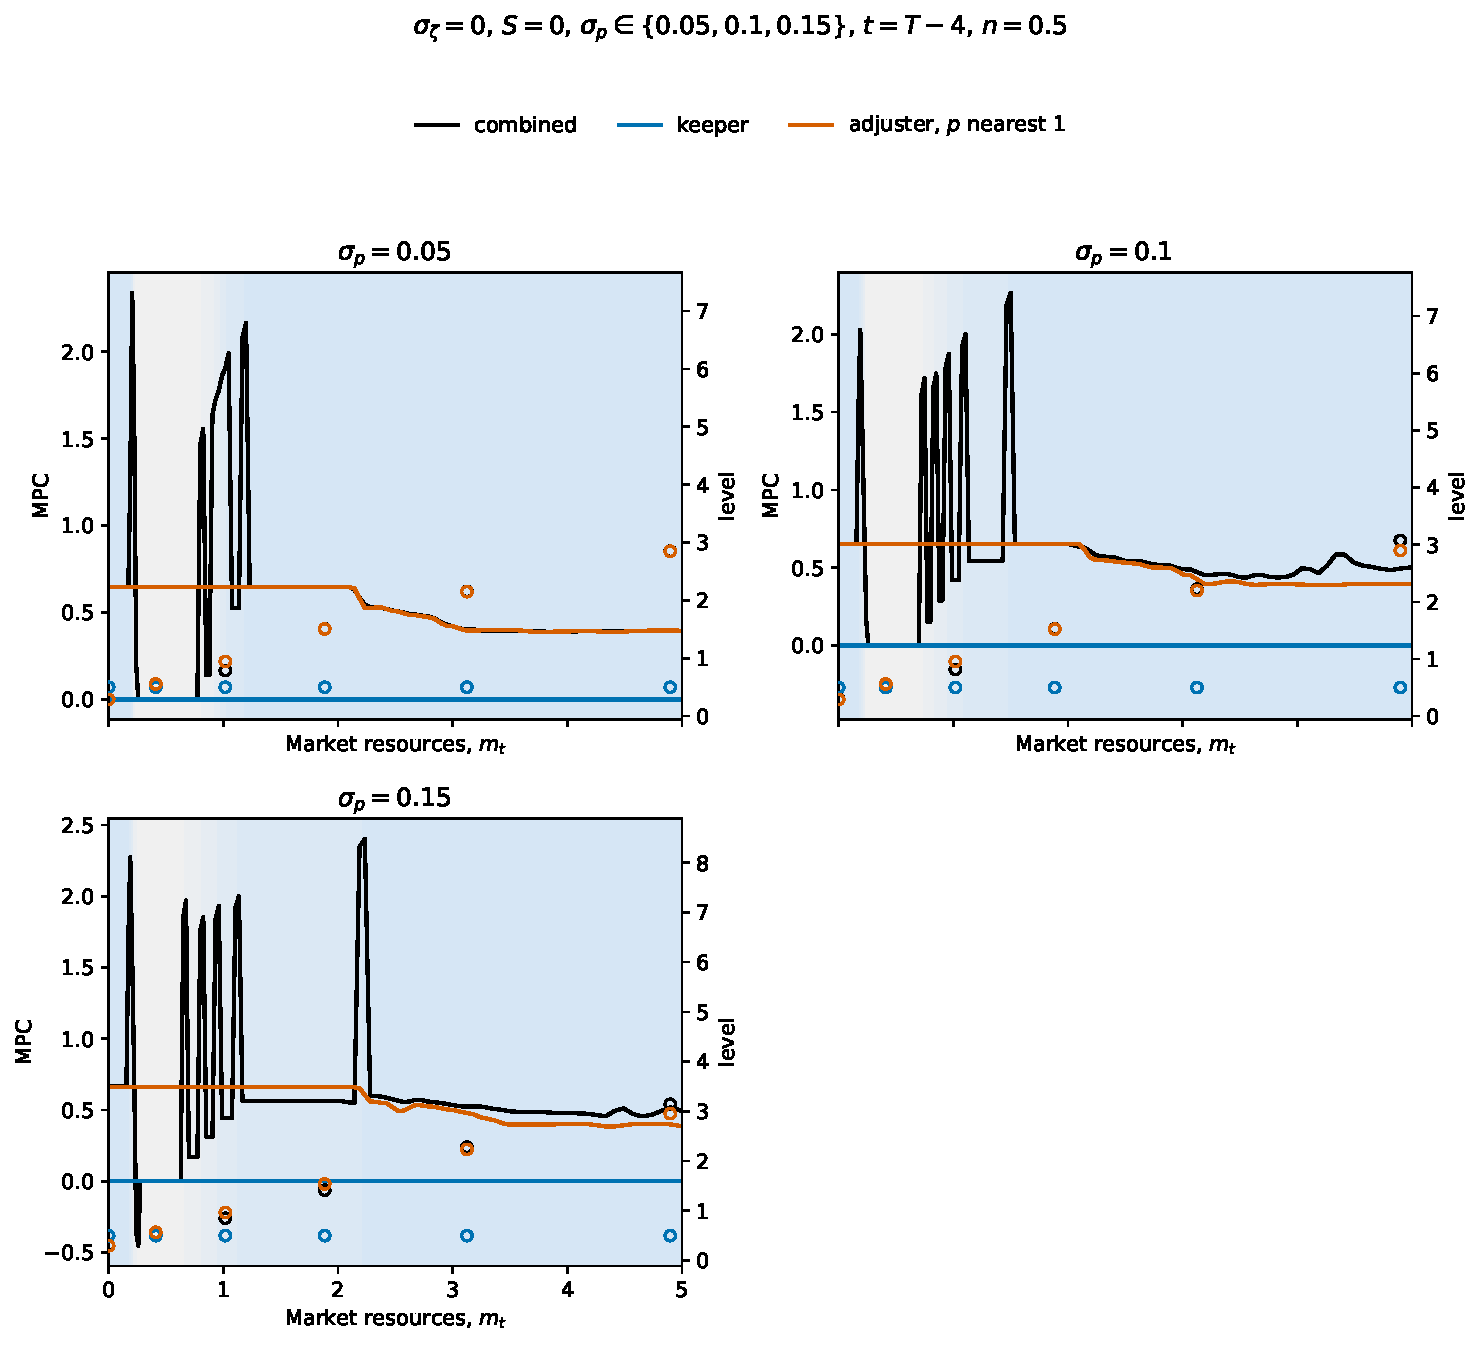
\includegraphics[width=\linewidth]{../Figures/DurableModel/PriceStd_d_periodt_MPC_decomp.pdf}
		\caption{MPC decomposition of durable consumption $d_t(n_t,m_t)$.}
		\label{fig:PriceStd_d_periodt_MPC_decomp}
	\end{subfigure}
	\caption{MPC and policy functions of non-durable and durable consumption using stochastic prices.}
	\label{fig:PriceStd_periodt_MPC_decomp}
\end{figure}


\begin{figure}[htbp]
	\centering
	\begin{subfigure}{0.48\textwidth}
		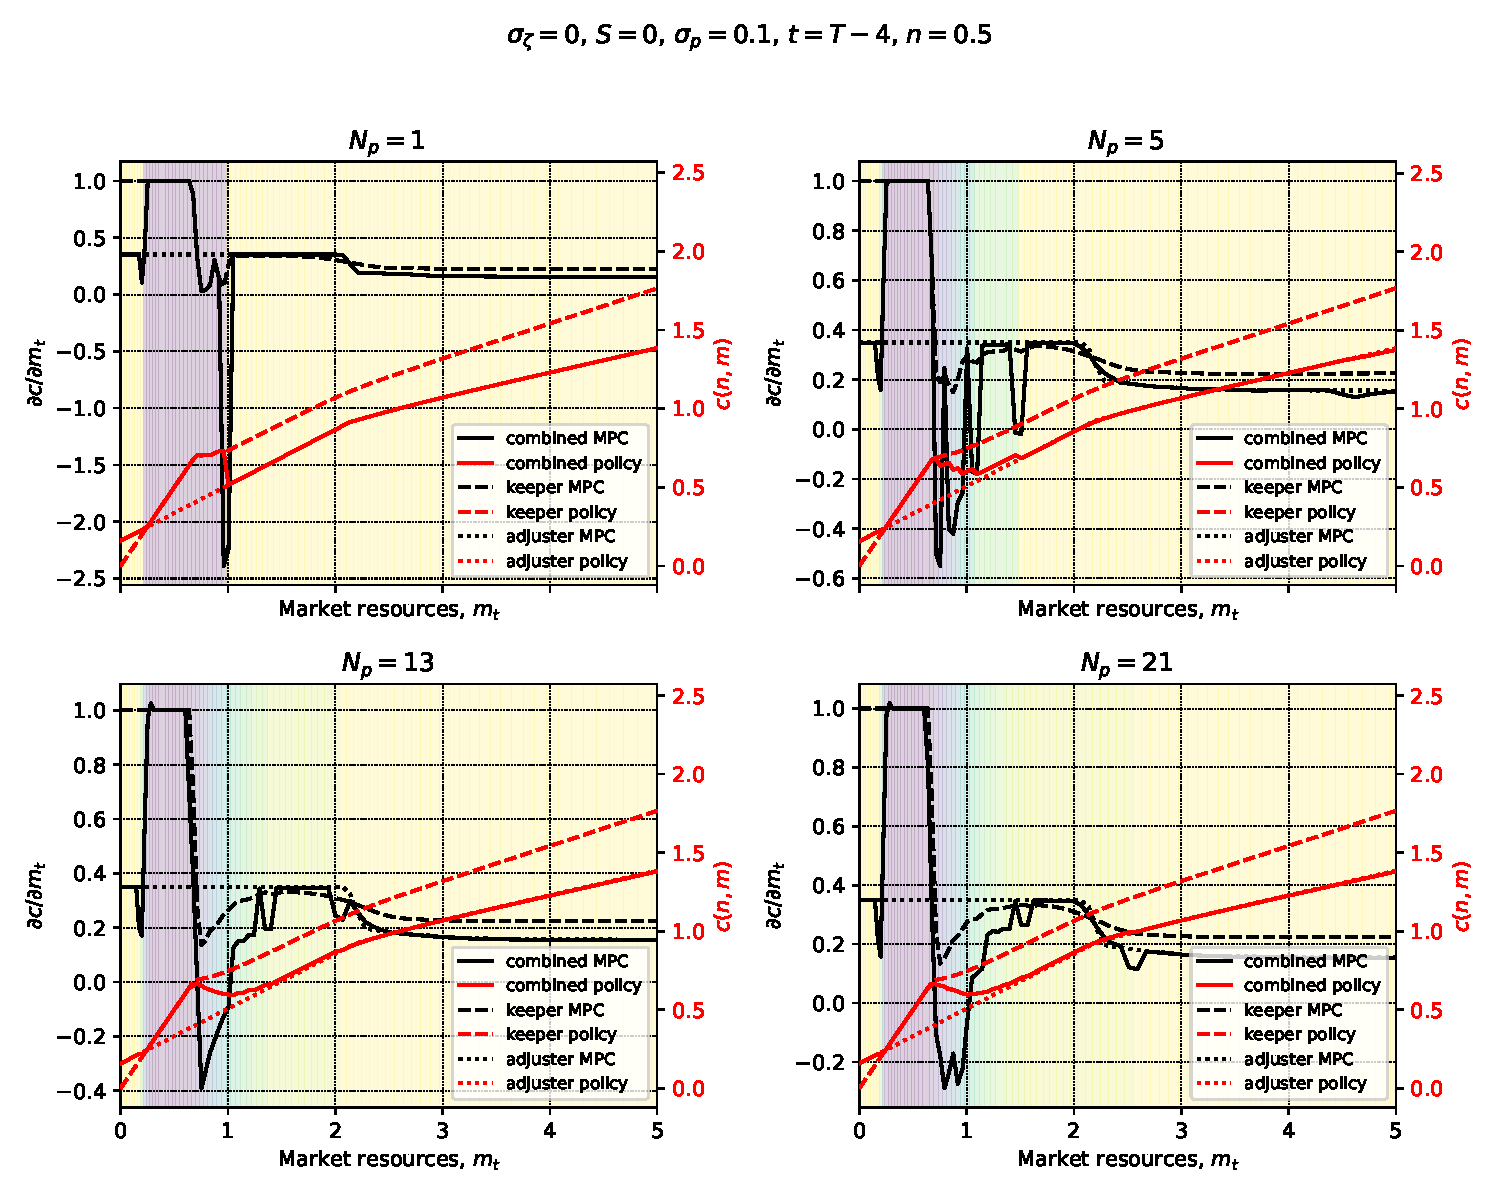
\includegraphics[width=\linewidth]{../Figures/DurableModel/PriceCount_c_periodt_MPC_decomp.pdf}
		\caption{MPC decomposition of nondurable consumption $c_t(n_t,m_t)$.}
		\label{fig:PriceCount_c_periodt_MPC_decomp}
	\end{subfigure}
	\hfill
	\begin{subfigure}{0.48\textwidth}
		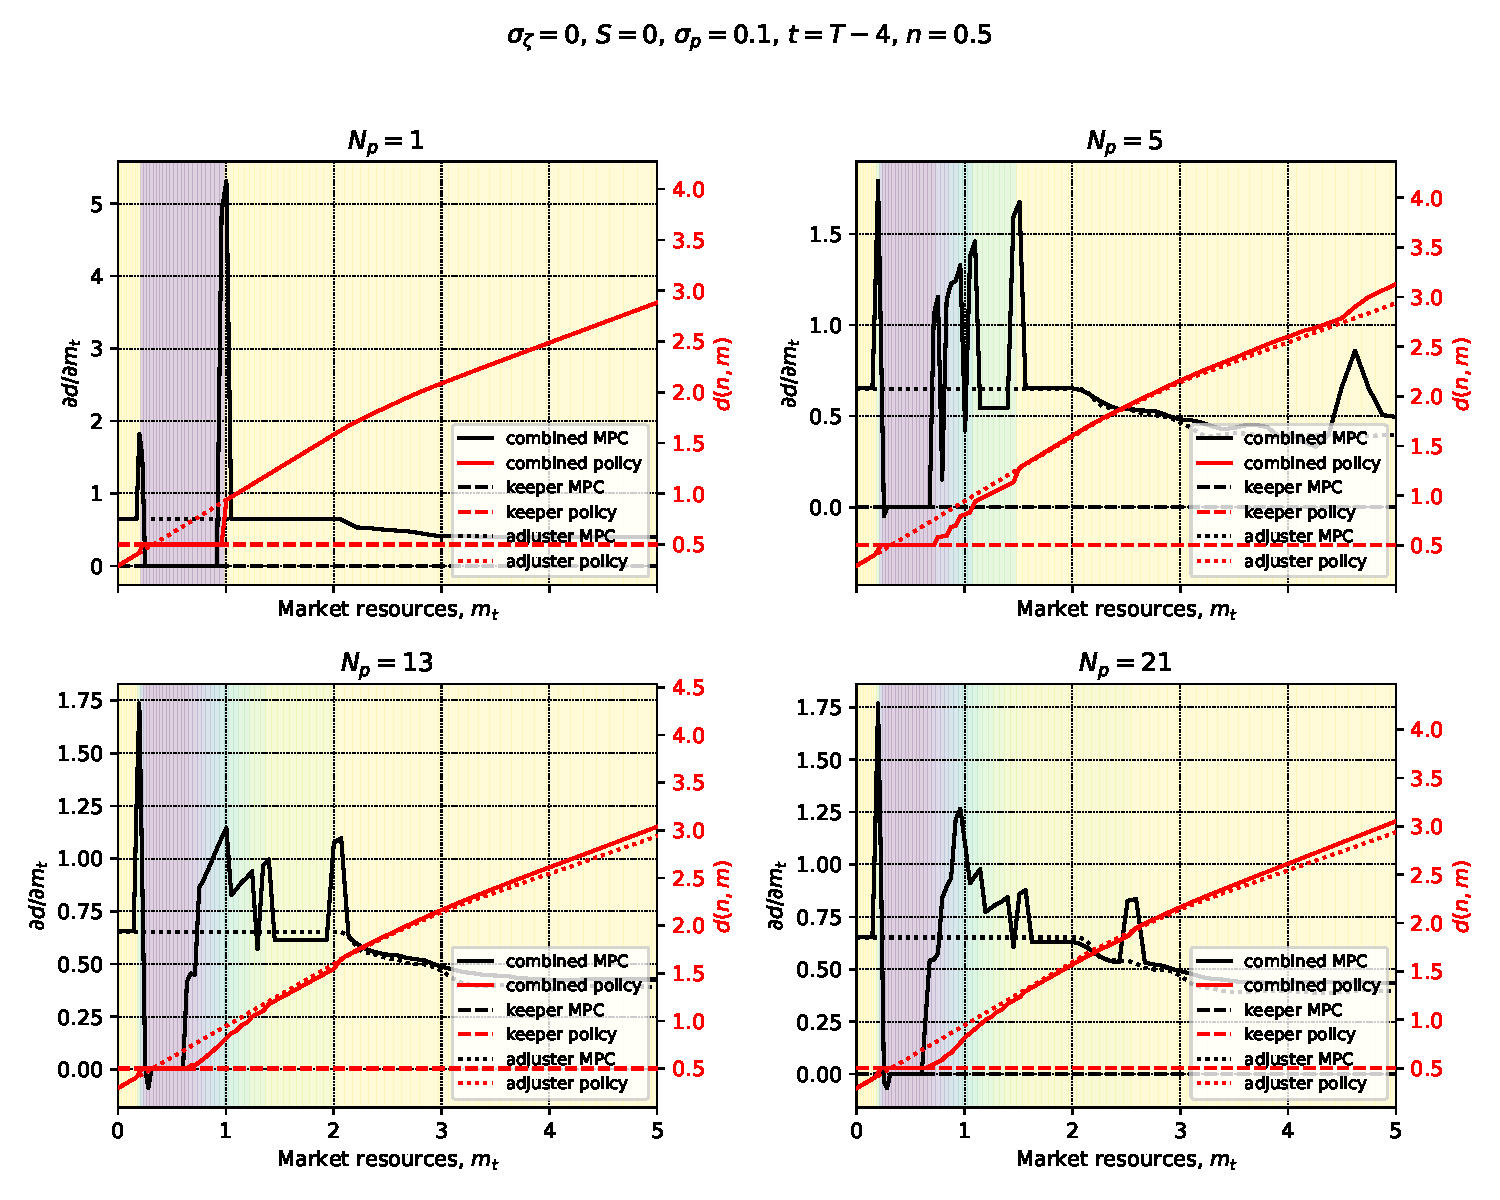
\includegraphics[width=\linewidth]{../Figures/DurableModel/PriceCount_d_periodt_MPC_decomp.pdf}
		\caption{MPC decomposition of durable consumption $d_t(n_t,m_t)$.}
		\label{fig:PriceCount_d_periodt_MPC_decomp}
	\end{subfigure}
	\caption{MPC and policy functions of non-durable and durable consumption varying the number of price points.}
	\label{fig:PriceCount_periodt_MPC_decomp}
\end{figure}


\subsection{Extension: Search and Stochastic Prices}\label{subsec:ModelBasicFull}

This subsection nests the search frictions of Section~\ref{subsec:ModelBasicSearch} with the stochastic durable prices of Section~\ref{subsec:ModelBasicPrice}. Extreme Value Type I taste shocks (Section~\ref{subsec:ModelBasicTaste}) and directed search are alternative ways of smoothing the keep-versus-adjust margin; nesting both would double-smooth the discrete choice without a clear economic interpretation, so the nested environment uses search rather than EV Type I shocks, together with price risk on the adjuster's continuous problem.

The household faces an idiosyncratic relative price $p_t$ at which new durables can be purchased and chooses a search intensity $\varepsilon_t\in[0,1]$ that determines the probability of successfully adjusting, at convex cost $\sigma(\varepsilon_t)$ from equation~\eqref{eq:search_cost_basic}. The price is independent of income,
\begin{align}
	\log p_t &\sim \mathcal{N}\Big(-\frac{\sigma_p^2}{2},\,\sigma_p^2\Big), \qquad \mathbb{E}[p_t]=1, \label{eq:full_p_dist}
\end{align}
with $p_t\perp\theta_t$ and i.i.d.\ across periods.

The within-period timeline is as follows. After $\theta_t$ has materialized and $(m_t,n_t)$ are known, the household observes $p_t$. Liquidity upon adjustment remains $\ell_t=m_t+(1-\tau)n_t$, independent of the price. The keeper's problem is unaffected by $p_t$, so $v_t^{\text{keep}}(m_t,n_t)$ retains its baseline Bellman definition. The adjuster's budget constraint is the price-contingent constraint~\eqref{eq:price_budget}, so the adjuster's conditional value $v_t^{\text{adj}}(\ell_t,p_t)$ and its continuous policies $c_t^{\text{adj}}(\ell_t,p_t)$, $d_t^{\text{adj}}(\ell_t,p_t)$ are exactly as in Section~\ref{subsec:ModelBasicPrice}. Given these two conditional values, the household chooses search intensity to maximize the price-contingent objective
\begin{align}
	v_t(m_t,n_t,p_t)
	&= \max_{\varepsilon_t\in[0,1]}
	\Big[(1-\varepsilon_t)\, v_t^{\text{keep}}(m_t,n_t)
	+ \varepsilon_t\, v_t^{\text{adj}}(\ell_t,p_t)
	- \sigma(\varepsilon_t)\Big]. \label{eq:full_discrete}
\end{align}
Equation~\eqref{eq:full_discrete} nests the standalone search and price extensions as special cases: with $\sigma_p\to 0$ it collapses to the search problem~\eqref{eq:search_discrete_basic}; with $S\to 0$ it collapses to the price-contingent hard maximum~\eqref{eq:price_discrete}; and with both limits simultaneous it collapses to the hard-maximum baseline of Section~\ref{sec:ModelBasic}.

Because $p_{t+1}$ is drawn afresh every period, the object that enters today's Euler equations is the price-integrated value function
\begin{align}
	\bar v_t(m_t,n_t)
	&\equiv \mathbb{E}_{p_t}\big[v_t(m_t,n_t,p_t)\big], \label{eq:full_barv}
\end{align}
which replaces $v_t(m_t,n_t)$ inside the Bellman equations for $v_{t-1}^{\text{keep}}$ and $v_{t-1}^{\text{adj}}$. The two frictions play complementary roles: $p_t$ shifts the adjuster's continuous problem and therefore the level of $v_t^{\text{adj}}$; and $\varepsilon_t^\ast$ translates the resulting gap $v_t^{\text{adj}}-v_t^{\text{keep}}$ into a smooth probability of adjusting. I derive the optimal search-effort rule, the combined envelope conditions, the Euler equations, the terminal-period solution, and the EGM algorithm for the nested model in appendix~\ref{subsec:appdx_full_basic}.

Using a combination of endogeneous search and stochastic prices can smooth policy functions when searchfrictions are not enough. Figure~\ref{fig:pricestd_search_Ss_T} illustrates the S,s region for the terminal period, and figure~\ref{fig:PriceStd_Search_periodt_MPC_decomp} shows the MPCs in period t.


\begin{figure}[htbp]
	\centering
	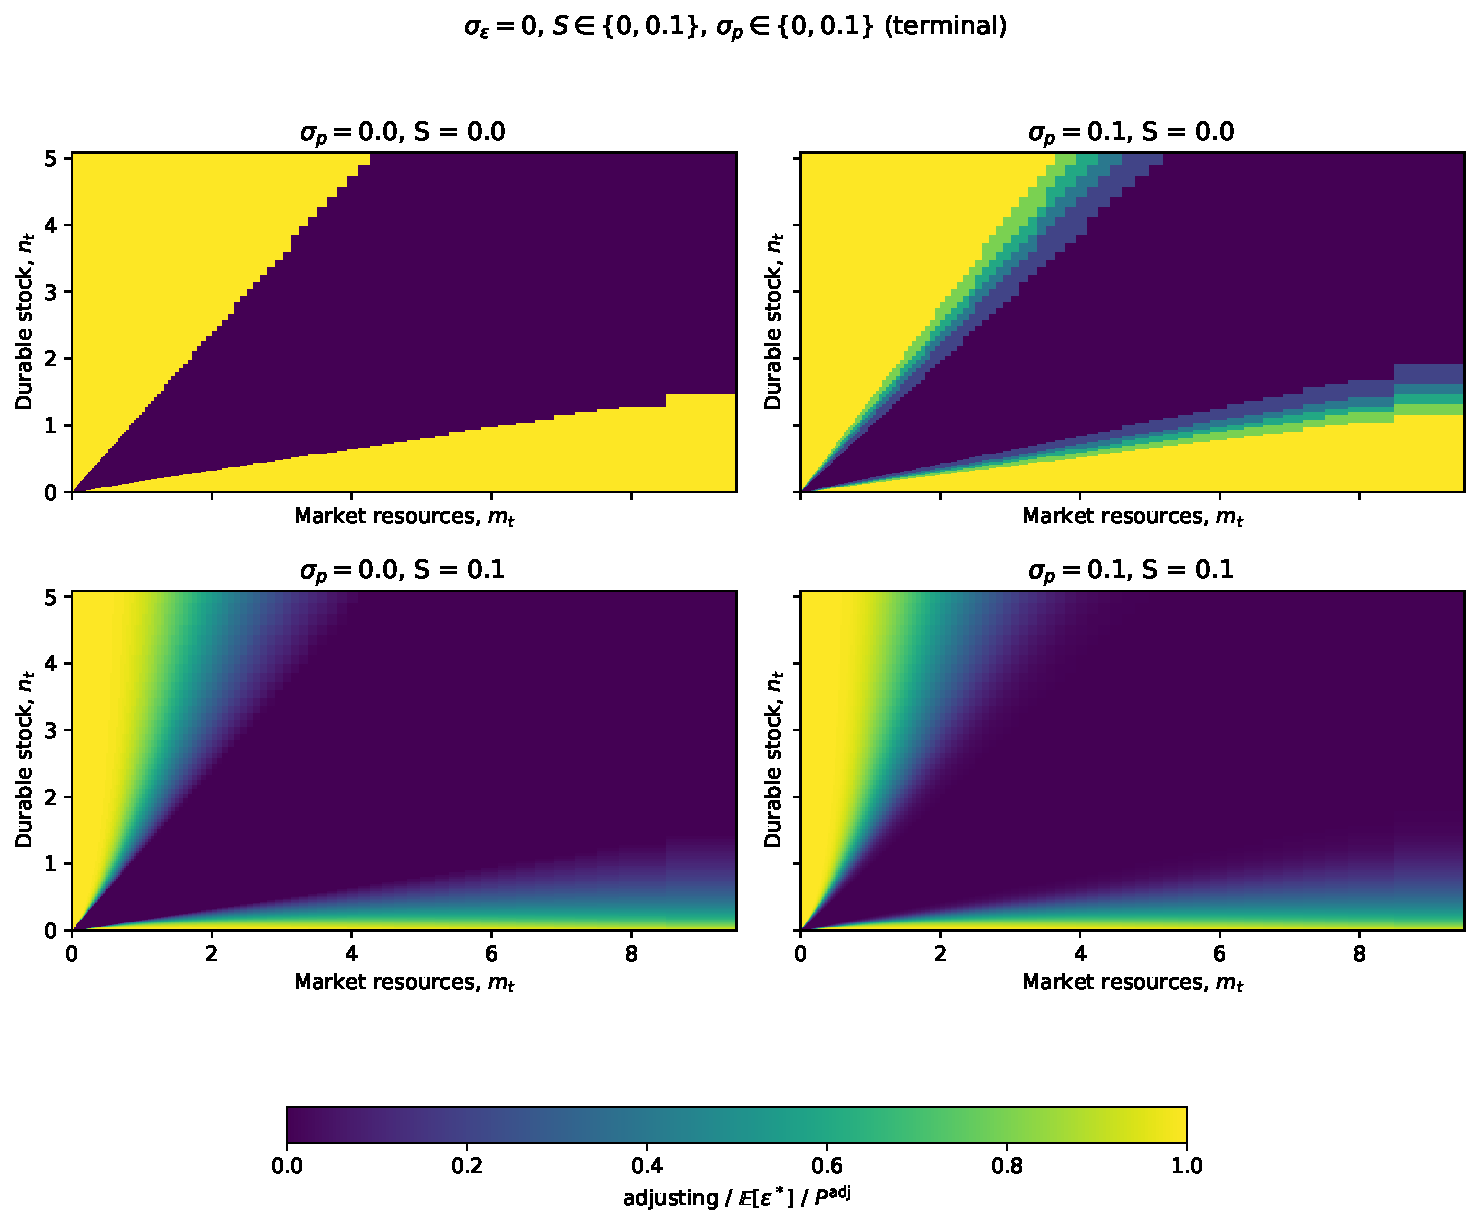
\includegraphics[width=0.85\linewidth]{../Figures/DurableModel/PriceStd_Search_Ss_T.pdf}
	\caption{Adjustment regions in period $T$ under stochastic durable prices and endogeneous search.}
	\label{fig:pricestd_search_Ss_T}
\end{figure}


\begin{figure}[htbp]
	\centering
	\begin{subfigure}{0.48\textwidth}
		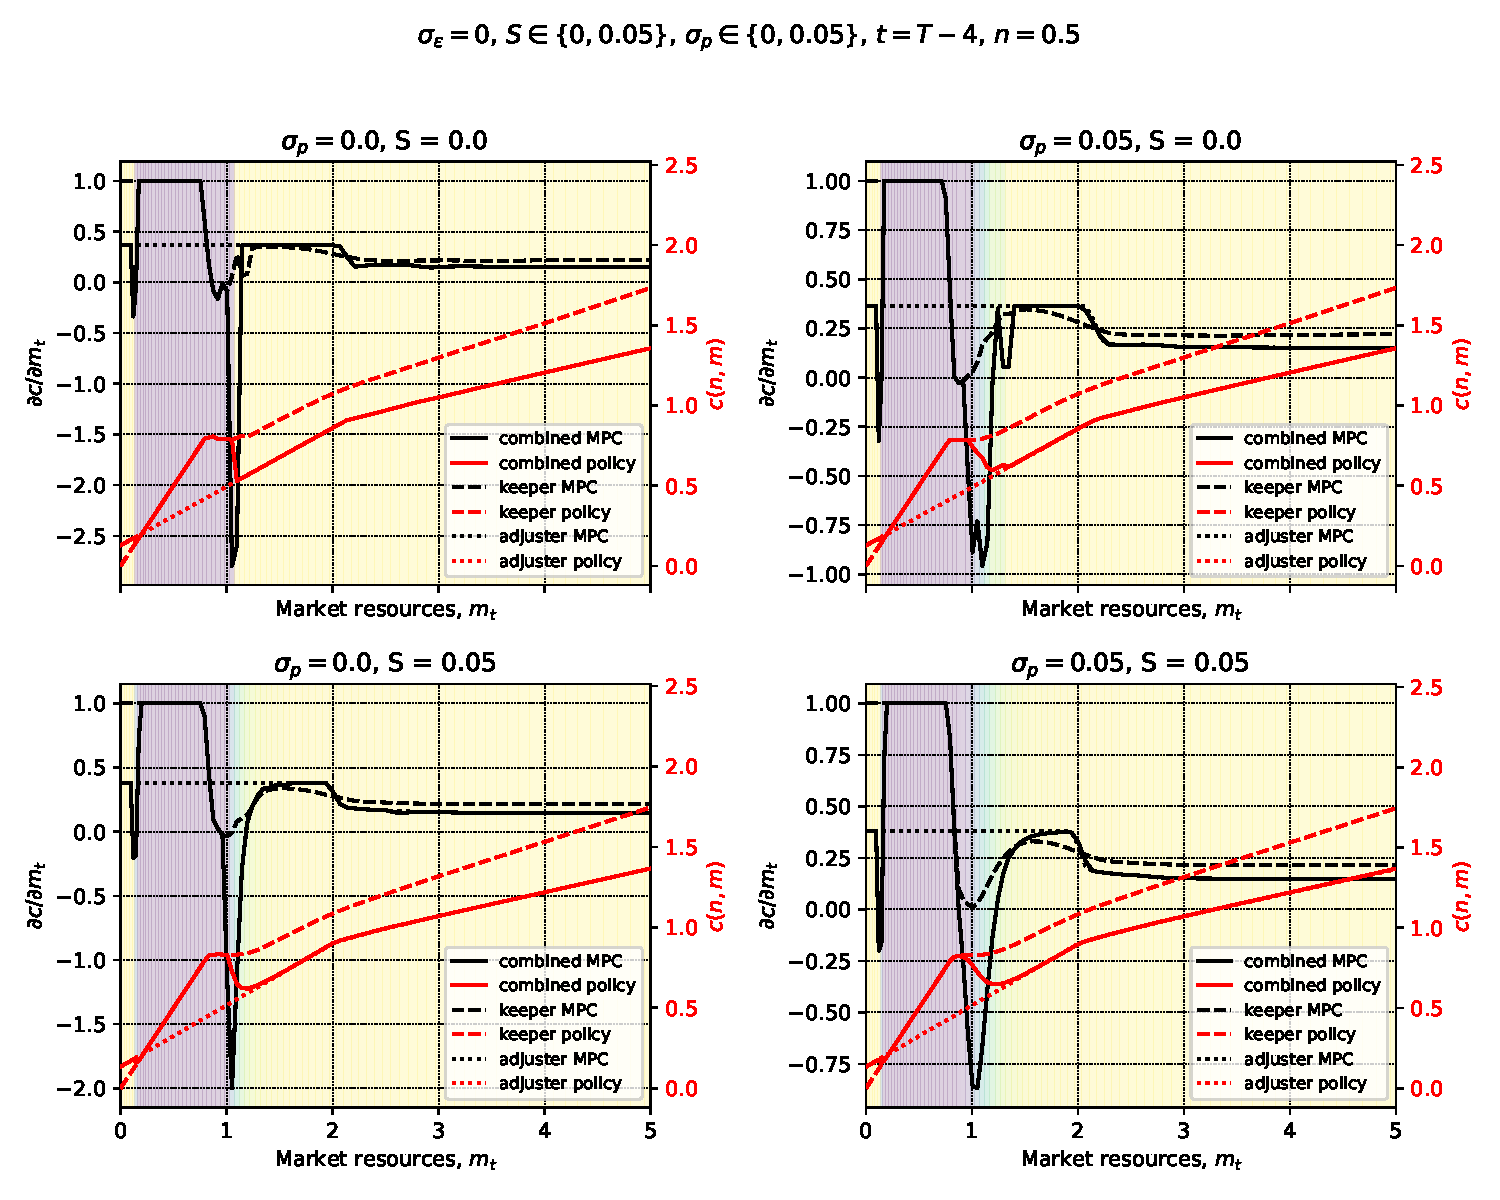
\includegraphics[width=\linewidth]{../Figures/DurableModel/PriceStd_Search_c_periodt_MPC_decomp.pdf}
		\caption{MPC decomposition of nondurable consumption $c_t(n_t,m_t)$.}
		\label{fig:PriceStd_Search_c_periodt_MPC_decomp}
	\end{subfigure}
	\hfill
	\begin{subfigure}{0.48\textwidth}
		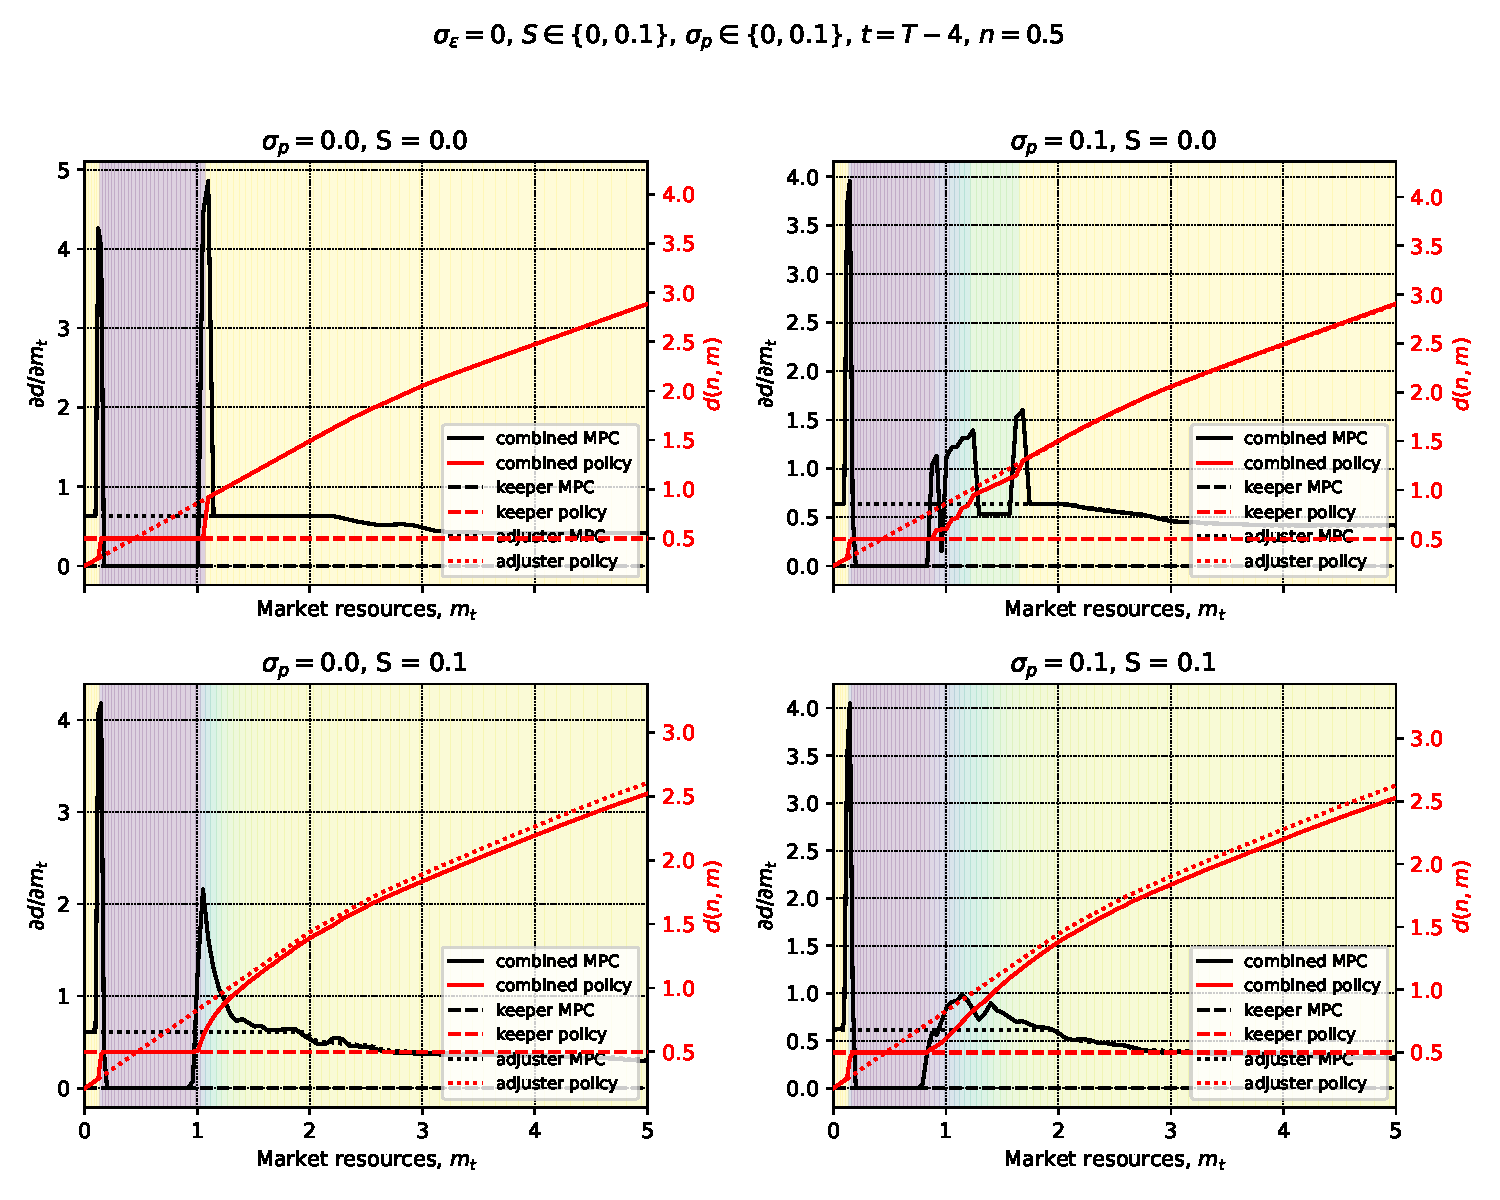
\includegraphics[width=\linewidth]{../Figures/DurableModel/PriceStd_Search_d_periodt_MPC_decomp.pdf}
		\caption{MPC decomposition of durable consumption $d_t(n_t,m_t)$.}
		\label{fig:PriceStd_Search_d_periodt_MPC_decomp}
	\end{subfigure}
	\caption{MPC and policy functions of non-durable and durable consumption using stochastic prices and search.}
	\label{fig:PriceStd_Search_periodt_MPC_decomp}
\end{figure}
